\usepackage[T1]{fontenc}
\usepackage{newtxtext}       % 
\usepackage[varvw]{newtxmath}       % selects Times Roman as basic font

\usepackage{graphicx}
% unless \nofake is defined, render graphics that are available, and draw
% missing ones (e.g., figures from paper branch submodules) as black boxes,
% like graphicx's demo option
\makeatletter
\newif\iffake@found
\def\fake@checkgraphic#1{%
  \global\fake@foundfalse
  \begingroup
  \ifx\Ginput@path\@undefined\else\let\input@path\Ginput@path\fi
  \filename@parse{#1}%
  \ifx\filename@ext\relax
    \@for\fake@ext:=\Gin@extensions\do{%
      \iffake@found\else
        \IfFileExists{\filename@area\filename@base\fake@ext}%
          {\global\fake@foundtrue}{}%
      \fi}%
  \else
    \IfFileExists{#1}{\global\fake@foundtrue}{}%
  \fi
  \endgroup}
\ifdefined\nofake\else
\AtBeginDocument{%
  \let\fake@Ginclude@graphics\Ginclude@graphics
  \def\Ginclude@graphics#1{%
    \fake@checkgraphic{#1}%
    \iffake@found
      \fake@Ginclude@graphics{#1}%
    \else
      \rule{\@ifundefined{Gin@@ewidth}{150pt}{\Gin@@ewidth}}%
      {\@ifundefined{Gin@@eheight}{100pt}{\Gin@@eheight}}%
    \fi}}
\fi
\makeatother

\usepackage[utf8]{inputenc}

\usepackage[export]{adjustbox}
\usepackage{algorithm}
% \usepackage{algorithmic}
% \usepackage[algcompatible]{algpseudocode}
\usepackage{algorithmicx,algpseudocode}
\usepackage{amsmath,amsfonts}
\usepackage{array}
\usepackage{bibunits}
\usepackage{booktabs}
\usepackage{caption}
\usepackage{cite}
\usepackage{colortbl}
\usepackage{csvsimple}
\usepackage{etoolbox}
\usepackage[T1]{fontenc} % adapted from https://tex.stackexchange.com/a/388208
\usepackage[margin=1in]{geometry}
\usepackage{graphicx}
\usepackage{glossaries,glossaries-extra}
\usepackage[hypertexnames=false]{hyperref}
\usepackage{cleveref}
\usepackage{ifthen}
\usepackage{import}
\usepackage{listings}
\usepackage{longtable}
\usepackage{makecell}
\usepackage{makecmds}
\usepackage{multirow}
\usepackage{natbib}
\usepackage[section]{placeins}
\usepackage{pythonhighlight}
\usepackage{rotating}
\usepackage[moderate]{savetrees}
\usepackage{setspace}
\usepackage{siunitx}
\usepackage{stringstrings}
\usepackage{subcaption}
\usepackage{subcaption}
\usepackage{tabularx}
\usepackage{textcomp}
\usepackage{vcell}
\usepackage{xcolor}
\usepackage{xfp}
\usepackage{xparse}
\usepackage{xstring}

\newcommand*\Let[2]{\State #1 $\gets$ #2}
\renewcommand{\algorithmicrequire}{\textbf{Input:}}
\renewcommand{\algorithmicensure}{\textbf{Output:}}
\newcommand{\ceil}[1]{\left\lceil #1 \right\rceil}

% pragma once, adapted from https://tex.stackexchange.com/a/195173
\makeatletter
\let\pragma@iinput=\@iinput
\def\@iinput#1{\xdef\@pragmafile{#1}\pragma@iinput{#1} }
\def\@pragmafile{default}
\def\pragmaonce{%
   \csname pragma@\@pragmafile\endcsname
   \global\expandafter\let \csname pragma@\@pragmafile\endcsname = \endinput
}
\makeatother

% adapted from https://www.siam.org/Portals/0/Macros/Standard/docsiamart.pdf
\Crefname{ALC@unique}{Line}{Lines}

\ifdefined\nodraft
\else
\usepackage{draftwatermark}
\usepackage{lineno}
\linenumbers
\renewcommand{\linenumberfont}{\normalfont\small\color{red}}
\fi

\defaultbibliography{bibl}
\defaultbibliographystyle{apalike}

% figure submodules live in the paper branch, which builds this document via \import{tex/}
\graphicspath{{./}{./tex/}{./hereditary-stratigraph-concept/tex}{./hstrat-evolutionary-inference}}

% \newtheorem{theorem}{Theorem}


\makeglossaries

\newglossaryentry{differentia}
{
    name=differentia,
    description={randomly generated information that can be used to differentiate two strata at the same layer (with a probability of spurious collision)}
}

\newglossaryentry{stratum}
{
    name=stratum,
    description={differentia container associated with a particular historical stage}
}

\newglossaryentry{deposit}
{
    name=deposit,
    description={the act of extending the historical record with a new stratum}
}

\newglossaryentry{deposition}
{
    name=deposition,
    description={the stratum appended to the historical record}
}

\newglossaryentry{time point}
{
    name=time point,
    description={refers to the stage where a specific number of depositions have taken place}
}

\newglossaryentry{deposition time}
{
    name=deposition time,
    description={refers to the time point at which a stratum was deposited, zero indexed}
}

\newglossaryentry{genesis}
{
    name=genesis,
    description={the time point associated with the first stratum deposition}
}

\newglossaryentry{time}
{
    name=time,
    description={number of depositions elapsed between two time points}
}

\newglossaryentry{layer age}
{
    name=layer age,
    description={the number of depositions elapsed since a layer's deposition time}
}

\newglossaryentry{record depth}
{
    name=record depth,
    description={the number of depositions elapsed onto the historical record --- the number of layers within a historical record}
}

\newglossaryentry{layer}
{
    name=layer,
    description={position within a historical record associated with a single time point, which may or may be occupied}
}

\newglossaryentry{retained/pruned layer}
{
    name=retained/pruned layer,
    description={a layer within a historical record with present/removed strata, respectively}
}

\newglossaryentry{layer time point}
{
    name=layer time point,
    description={the deposition time associated with a layer}
}

\newglossaryentry{pruning}
{
    name=pruning,
    description={deletion of strata from a historical record (i.e., to reduce space occupied by the record) --- also used to refer to deletion of perfect tracking records for extinct lineages,}
}

\newglossaryentry{retention}
{
    name=retention,
    description={the act of carrying over a stratum into the next time point during the stratum deposition process}
}

\newglossaryentry{gap}
{
    name=gap,
    description={layers associated with contiguous time points that have been pruned ---- introduces inference uncertainty when comparing two columns}
}

\newglossaryentry{gap width}
{
    name=gap width,
    description={the number of contiguous time points that have been pruned --- gap with increases inference uncertainty}
}

\newglossaryentry{sparse/dense retention}
{
    name=sparse/dense retention,
    description={refers to relatively wide or relatively tight gap width, respectively}
}

\newglossaryentry{gap width distribution}
{
    name=gap width distribution,
    description={how gap widths relate to layer deposition times}
}

\newglossaryentry{resolution}
{
    name=resolution,
    description={the width of the gap containing a pruned layer or immediately following a retained layer (may be zero in the case of two successive retained strata)}
}

\newglossaryentry{stratum retention policy algorithm}
{
    name=stratum retention policy algorithm,
    description={the decision-making procedure of which strata to prune at each time point (also referred to simply as ``policy'')}
}

\newglossaryentry{policy resolution guarantee}
{
    name=policy resolution guarantee,
    description={upper bounds on resolutions across layers of a historical record with respect to layer age and/or record depth}
}

\newglossaryentry{extant record size}
{
    name=extant record size,
    description={the quantity of strata retained within a historical record at a particular time point}
}

\newglossaryentry{extant record order of growth}
{
    name=extant record order of growth,
    description={the asymptotic scaling relationship between the extant record size and record depth}
}

\newglossaryentry{pruning enumeration}
{
    name=pruning enumeration,
    description={calculation of the set of strata to be pruned at a particular time point under a retention policy}
}

\newglossaryentry{policy enactment}
{
    name=policy enactment,
    description={the act of performing pruning enumeration and deleting strata with enumerated deposition times}
}

\newglossaryentry{update}
{
    name=update,
    description={the process of performing a deposition and applying policy enactment}
}

\newglossaryentry{update time complexity}
{
    name=update time complexity,
    description={the scaling relationship associated with the number of computational operations necessary to perform an update}
}

\newglossaryentry{founding stratum}
{
    name=founding stratum,
    description={the first stratum deposited into the historical record, the oldest stratum}
}

\newglossaryentry{newest stratum}
{
    name=newest stratum,
    description={the most recent stratum deposited into the historical record}
}

\newglossaryentry{extant record}
{
    name=extant record,
    description={the set of strata that have been retained through the policy at the present time point}
}

\newglossaryentry{extant record enumeration}
{
    name=extant record enumeration,
    description={calculation of deposition times present in the extant record at a time point under a retention policy}
}

\newglossaryentry{policy self-consistency}
{
    name=policy self-consistency,
    description={the requirement for each deposition time within an extant record enumeration to be consistently present in all extant enumerations since that deposition time}
}

\newglossaryentry{historical record}
{
    name=historical record,
    description={refers to the set of layers defined up to the current time point, also referred to as a ``record''}
}

\newglossaryentry{hereditary stratigraphic column}
{
    name=hereditary stratigraphic column,
    description={container for a historical record --- in phylogenetic applications, associated with a digital population member, also referred to as a ``column''}
}

\newglossaryentry{annotation}
{
    name=annotation,
    description={the one-to-one association of hereditary stratigraphic records with individual digital organisms to facilitate phylogenetic analysis}
}

\newglossaryentry{inheritance}
{
    name=inheritance,
    description={the act of copying the parent organism's hereditary stratigraphic column annotation and performing an update to create the offspring organism's hereditary stratigraphic column annotation during a reproduction event}
}

\newglossaryentry{inference}
{
    name=inference,
    description={best-effort estimation of historical phylogenetic relationships from extant hereditary stratigraphic columns}
}

\newglossaryentry{perfect tracking}
{
    name=perfect tracking,
    description={maintenance of an exact record of phylogenetic events during an evolutionary simulation}
}

\newglossaryentry{streaming disposal problem}
{
    name=streaming disposal problem,
    description={poses the question of how to satisfactorily maintain a temporally representative collection of stored observations on a rolling basis as new observations stream in}
}



\begin{document}

\title{ Analysis of Phylogeny Tracking Algorithms for Serial and Multiprocess Applications }

\author{Matthew Andres Moreno\inst{1,2,3} \and
Santiago Rodriguz Papa\inst{4} \and
Emily Dolson\inst{4,5}}
%
\authorrunning{M. Moreno et al.}
% First names are abbreviated in the running head.
% If there are more than two authors, 'et al.' is used.
%
\institute{Ecology and Evolutionary Biology, University of Michigan, Ann Arbor, United States \and
Center for the Study of Complex Systems, University of Michigan, Ann Arbor, United States
\email{morenoma@umich.edu}\\
 \and
 Michigan Institute for Data Science, University of Michigan, Ann Arbor, United States\\
 \and Department of Computer Science and Engineering, Michigan State University, East Lansing, United States \\
 \and
Ecology, Evolution, and Behavior, Michigan State University, East Lansing, United States \\ }

% \author{
%     Matthew Andres Moreno\textsuperscript{1,2,3} \thanks{Corresponding author: \texttt{morenoma@umich.edu}} \quad
%     Santiago Rodriguez Papa\textsuperscript{4} \quad
%     Emily Dolson\textsuperscript{4,5} \quad
% }
% \date{}

% \newcommand{\affil}[1]{\textsuperscript{#1}}
% \newcommand{\affiliations}{
% \affil{1} Ecology and Evolutionary Biology, University of Michigan, Ann Arbor, United States \\
% \affil{2} Center for the Study of Complex Systems, University of Michigan, Ann Arbor, United States \\
% \affil{3} Michigan Institute for Data Science, University of Michigan, Ann Arbor, United States
% \affil{4} Department of Computer Science and Engineering, Michigan State University, East Lansing, United States \\
% \affil{5} Ecology, Evolution, and Behavior, Michigan State University, East Lansing, United States \\
% }

\maketitle

% \begin{center}
% \affiliations
% \end{center}

\begin{abstract}

% TODO we should probably use the word near optimal somewhere

% Reconstruction of phylogenetic history from natural biosequences kindles an evergreen profusion of statistical and algorithmic innovation because it is interesting and useful but especially because it is hard.
% Reconstruction of phylogenetic history from biological sequences raises a vast array of statistical and algorithmic challenges, because it is both important and difficult.
% Efforts to reconstruct phylogenetic history from biological sequences have proven a rich and enduring well for statistical and algorithmic innovation.
Since the advent of modern bioinformatics, the challenging, multifaceted problem of reconstructing phylogenetic history from biological sequences has hatched perennial statistical and algorithmic innovation.
Studies of the phylogenetic dynamics of digital, agent-based evolutionary models motivate a peculiar converse question: how to best engineer tracking to facilitate fast, accurate, and memory-efficient lineage reconstructions?
Here, we formally describe procedures for phylogenetic analysis in both serial and distributed computing scenarios.
With respect to the former, we demonstrate reference-counting-based pruning of extinct lineages.
For the latter, we introduce a trie-based phylogenetic reconstruction approach for ``hereditary stratigraphy'' genome annotations.
This process allows phylogenetic relationships between genomes to be inferred by comparing their similarities, akin to reconstruction of natural history from biological DNA sequences.
Phylogenetic analysis capabilities significantly advance distributed agent-based simulations as a tool for evolutionary research, and also benefit application-oriented evolutionary computing.
Such tracing could also extend to other digital artifacts that proliferate through replication, like digital media and computer viruses.


% This issue directly implicates the design of virtual annotations on digital genomes to facilitate post-hoc inference — and analysis — of their lineages.
% Virtual annotations on digital genomes have been designed to solve this issue by facilitating post-hoc inference — and analysis — of their lineages.
% This emerging so-called ``hereditary stratigraphy’’ methodology abstracts this problem to a more general one: how to satisfactorily maintain a temporally representative collection of observations that stream in on a rolling basis.
% We term this more general question the ``streaming curation problem.’’
% Because ongoing data feeds necessitate continual downsampling when faced with storage and memory limitations, the streaming curation problem occurs also in context of unattended data loggers, irregularly-uplinked wireless sensor network devices, and servers under continuous application monitoring, among other scenarios.
% To meet requirements of diverse streaming curation scenarios, we present a suite of streaming curation policy algorithms that trade off along a continuum of collection size and temporal coverage.
% Policies span $\mathcal{O}(n)$, $\mathcal{O}(\log n)$, and $\mathcal{O}(1)$ orders of growth in curated collection size.
% Within each order of growth, policy algorithms differ in relative prioritization of newer versus older data.
% We explore two alternatives: even density distribution across history or recency-proportional distribution with greater density at more recent time points.
% Policy algorithm designs explicitly pre-determine retained collection composition at each time point, enabling key optimizations to reduce storage overhead and streamline processing of incoming observations.

% Hereditary stratigraphy’s application of streaming curation to lineage inference arises through interpretation of each individual as an independent observation of lineage association within an ongoing generational stream.
% Replicator annotations operationalize this abstract interpretation.
% % Each replicator is adjoined with a heritable set of checkpoint identifiers.
% Each replicator is given a heritable set of checkpoint identifiers.
% New checkpoints are created each generation, and streaming curation policy algorithms decide which to retain.
% Recent experimental work applying this principle has yielded robust recovery of phylogenetic information.
% Here, we formalize the theoretical foundations of hereditary stratigraphy through exposition of streaming curation algorithms.
% % and resolve a lynchpin limitation to its end-to-end application: methods for scalable, whole-tree reconstruction from checkpoint annotations.
% As a point of comparison, we also provide formal analysis for existing centralized methods for direct phylogenetic tracking.
% Implications of underlying streaming curation algorithms extend more broadly still, encompassing wider issues of rolling record management.
\end{abstract}



\clearpage
\newpage

\begin{bibunit}

\section{Introduction} \label{sec:introduction}

Biological phylogenetic history is staggeringly vast and deep.
Prokaryotes alone have a contemporary population size on the order of $10^{30}$ cells \citep{whitman1998prokaryotes}, and the phylogenetic record stretches back on the order of billions of years \citep{arndt2012processes}.
In addition to addressing questions of natural history, access to the phylogenetic record of biological life has proven informative to conservation biology, epidemiology, medicine, and biochemistry among other domains \citep{faithConservationEvaluationPhylogenetic1992, STAMATAKIS2005phylogenetics, frenchHostPhylogenyShapes2023,kim2006discovery}.

Although trifling in scale by comparison, computer simulations of evolution can generate vast histories in their own right, with common agent-based models achieving on the order of 200 million replication cycles per day \citep{ofria2009artificial}.
Distillation of this onslaught of history is necessary for data management tractability \citep{dolson2020interpreting, ralph_efficiently_2020}.
Nonetheless, existing analyses of phylogenetic structure within digital systems have already proven valuable, enabling diagnosis of underlying evolutionary dynamics \citep{11007774,hernandez2022can,shahbandegan2022untangling, lewinsohnStatedependentEvolutionaryModels2023a} and even serving as a mechanism to guide evolution in application-oriented domains \citep{lalejini2024phylogeny,lalejini2024runtime,murphy2008simple,burke2003increased}.

Here, we formalize data structures and algorithmic procedures for space-efficient aggregation of phylogenetic history from evolutionary simulations on a rolling basis, and investigate their runtime performance characteristics.
% We focus in particular on asexual lineages, in which each entity has exactly one parent.
% Sexual lineages, in which entities may have more than one parent, are beyond the scope of this paper.
% They present unique challenges in phylogenetic tracking that merit methodological treatment in their own right \citep{godin2019apoget,moreno2024methods,mcphee2018detailed}.
In this paper, we focus in particular on asexual lineages, in which each entity has exactly one parent --- as opposed to sexual lineages (or Ancestral Recombination Graphs), in which entities may have more than one parent.
Although they have historically underpinned a substantial proportion of evolutionary computation and simulation systems \citep{koza1994genetic,jefferson1990evolution} and continue to be of great interest within the community \citep{dang2018escaping}, they present unique challenges in phylogenetic tracking that merit methodological treatment in their own right \citep{godin2019apoget,moreno2024methods,mcphee2018detailed}. Moreover, asexual lineages can serve as the basis for tracking recombination in that one strategy for doing so is to maintain a unique tree for each site in the genome.


%We cover two approaches: pruning of extinct lineages and coarsening of phylogenetic history.
%The former applies to direct tracking approaches and targets single-processor, serial simulation.
%The latter, in contrast, targets decentralized many-processor parallel/distributed simulation and involves a post hoc, reconstruction-based approach.

We cover two approaches: (1) tracking lineages directly using a centralized data structure and (2) a decentralized, reconstruction-based approach called hereditary stratigraphy.
The former approach allows perfect accuracy, and we show that it is efficient when targeting single-processor applications (\textit{i.e.} using serial simulation).
The latter, in contrast, was designed for decentralized many-processor parallel/distributed simulation.
It supports user-controlled trade-offs between reconstruction precision and runtime resource overhead (e.g., memory, bandwidth).
We expect that hereditary stratigraphy indeed performs best in parallel/distributed contexts.

Accompanying public-facing open source Python packages provide convenient, plug-and-play access to phylogenetic tracking methodology across simulation systems \citep{moreno2022hstrat,dolson2023phylotrackpy}.
In this manner, methods described here promise to --- and, indeed, already have --- directly enable simulation-based evolution research.
On a purely algorithmic level, procedures and, in particular, representational considerations involved in direct phylogenetic tracking pertain also to more general issues of phylogenetic computation.
% Likewise, data-management processes necessary to decentralized phylogenetic tracking relate directly to broader questions about on-the-fly binning within the domain of stream processing \citep{moreno2024algorithms}.
Likewise, data-management processes necessary to decentralized phylogenetic tracking relate directly to broader questions involving on-the-fly binning within the domain of stream processing \citep{moreno2024algorithms}.

Having motivated applications and algorithmic analyses of direct and decentralized tracking, we next present brief introductions to each methodology's operation.

\subsection{Direct Ancestry Tracking}

Most work on ancestry trees of self-replicating digital agents relies on centralized lineage tracking \citep{friggeri2014rumor,cohen1987computer,dolson2023phylotrackpy}.
% \footnote{A notable exception, \cite{libennowell2008tracing} exploit a serendipitous mechanistic opportunity to reconstruct global dissemination of chain emails.}
Direct approaches to tracking replicator provenance in digital systems operate on this graph structure directly, distilling it from the full set of parent-child relationships over the history of a population to produce an exact historical account.

Without further regard, naive complete lineage tracking performs poorly for large-scale evolutionary systems.
For long-lived simulations, practical memory limitations preclude comprehensive records of replication events, which accumulate linearly with elapsed generations and population size.
To achieve a tractable space complexity, extinct lineages can be pruned.
Within serial processing contexts, an efficient reference-counting based approach may be applied.
We discuss this technique further in Section \ref{sec:perfect-tracking-algorithm}.

\subsection{Decentralized Ancestry Tracking}

Unfortunately, computational scale --- i.e., parallel/distributed computing --- erodes the simplicity, efficiency, and effectiveness of centralized tracking.
Detecting lineage extinctions requires either (1) collation of all replication and destruction events to a centralized data store or (2) peer-to-peer transmission of extinction notifications that unwind a lineage's (possibly many-hop) trajectory across host nodes.
Both options introduce runtime communication overhead.
To boot, the perfect-tracking paradigm is fragile to data loss.
Even a single failed communication event can entirely disjoin knowledge of how large portions of phylogenetic history relate.
As data loss is ubiquitous at scale \citep{cappello2014toward,ackley2011pursue}, this limitation is of serious concern.

These concerns motivated development of \textit{hereditary stratigraphy}, an alternate, fully-decentralized approach to phylogenetic tracking \citep{moreno2022hereditary}.
This methodology uses special genome annotations, termed \textit{hereditary stratigraphic columns}.
These annotations facilitate fast, accurate post hoc inference of phylogenetic relationships among evolved agents, akin to how genetic material enables phylogenetic inference in biology.

The core mechanism of hereditary stratigraphy is accretion, and subsequent inheritance, of a new randomized data packet onto column annotations each generation.
These stochastic fingerprints, which we call ``differentia,'' serve as a sort of checkpoint for lineage identity at a particular generation.
At future time points, extant annotations will share identical differentia for the generations during which they experienced shared ancestry.
Thus, the first mismatched fingerprint between two annotations bounds the recency of their most recent common ancestor (MRCA).

To circumvent annotation size bloat, hereditary stratigraphy prescribes a ``pruning'' process to delete differentia on the fly as generations elapse.
This pruning, however, reduces precision of resulting phylogenies.
The last generation of common ancestry between two lineages can be resolved no finer than retained checkpoint times.
In the context of hereditary stratigraphy, we refer to the procedure for down sampling as a ``stratum retention algorithm'' and the resulting patterns of retained differentia as a ``stratum retention policy.''
Stratum retention algorithms must decide how many records to discard, but also how remaining records should be distributed over past time.
Tuning of stratum retention trade-offs is discussed in \citet{moreno2024algorithms} as an instance of the more general ``stream curation'' problem.
Here, we build on these results to discuss the use of hereditary stratigraphy specifically in a phylogenetic context.

% The primary additional complication that using hereditary stratigraphy for maintaining phylogenetic information adds over other use cases is the need to reconstruct the phylogeny at the end of a simulation.
A typical objective for phylogeny-oriented application of hereditary stratigraphy is synthesis of population-level ancestry history.
Although following from similar principles as pairwise MRCA estimation, procedures to reconstruct the ancestry tree of many stratigraph annotations merit some further elaboration.
Section \ref{sec:reconstruction-algorithm} provides an agglomerative, trie-based algorithm for this task.

\subsection{Outline}

Remaining exposition in this paper is structured as follows:
\begin{itemize}
% \item Section \ref{sec:methods} covers preliminaries and glossarizes key terminology,
\item Section \ref{sec:reconstruction-algorithm} contributes a recently-developed algorithm for full-tree reconstruction from hereditary stratigraphic annotation data and analyzes its runtime characteristics.
\item Section \ref{sec:perfect-tracking-algorithm} formally presents an algorithm for perfect phylogenetic tracking with analysis of its time and space complexity.
\item Section \ref{sec:discussion} discusses which situations better suit perfect tracking vs. hereditary stratigraphy.
% TODO do we need a results and discussion section???
% \item Section \ref{sec:results-and-discussion}
\item Section \ref{sec:conclusion} reflects on broader implications and future work.
% \item we include a Glossary of terminology related to hereditary stratigraphy, streaming curation, and phylogenetics in the Appendix.
\end{itemize}


% % \section{Preliminaries} \label{sec:methods}
% This section should introduce the necessary definitions, concepts, and notations that will be used throughout the paper.


% \section{Streaming Curation Algorithms} \label{sec:annotation-algorithms}

\input{lib/dissertationelse.tex}
\input{lib/dissertationonly.tex}

\begin{figure*}
  \centering
  \footnotesize
  \begin{tabular}{m{0.07\textwidth}@{}|c@{}|c@{\hskip 0.01\textwidth}|m{0.14\textwidth}}
%-------------------------------------------------------------------------------
\hspace{-1ex}Policy&Lower-Resolution Parameterization&Higher-Resolution Parameterization&\makecell[c]{Properties}\\\hline
%-------------------------------------------------------------------------------
    \rotatebox{90}{\textbf{Fixed Resolution}}
  &
    \makecell{
      \includegraphics[valign=t,width=0.3\textwidth]{submodules/hereditary-stratigraph-concept-binder/binder/retention-policies/teeplots/fixed_resolution=512+num_layers=1024+stratum_retention_predicate=fixed-resolution+viz=tweaked-stratum-retention-drip-plot+ext=}
    }
  &
    \makecell{
      \includegraphics[valign=t,width=0.3\textwidth]{submodules/hereditary-stratigraph-concept-binder/binder/retention-policies/teeplots/fixed_resolution=128+num_layers=1024+stratum_retention_predicate=fixed-resolution+viz=tweaked-stratum-retention-drip-plot+ext=}
    }
  &
  \makecell[{{p{0.14\textwidth}}}]{
  \centering
    \bf{Space Complexity}\\
    $\mathcal{O}(n)$\\
    \bf{MRCA Uncertainty}\\
    $\mathcal{O}(1)$
  }
  \makecell[{{p{0.14\textwidth}}}]{
  \raggedright
    where $n$ is gens elapsed.
  }\\\hline
%-------------------------------------------------------------------------------
    \adjustbox{
      minipage=10em,
      rotate=90,
    }{
      \centering
      \textbf{Depth-Proportional\\Resolution}
      \par
    }
  &
    \makecell{
      \includegraphics[valign=t,width=0.3\textwidth]{submodules/hereditary-stratigraph-concept-binder/binder/retention-policies/teeplots/guaranteed_depth_proportional_resolution=1+num_layers=1024+stratum_retention_predicate=depth-proportional-resolution+viz=tweaked-stratum-retention-drip-plot+ext=}
    }
  &
    \makecell{
      \includegraphics[valign=t,width=0.3\textwidth]{submodules/hereditary-stratigraph-concept-binder/binder/retention-policies/teeplots/guaranteed_depth_proportional_resolution=4+num_layers=1024+stratum_retention_predicate=depth-proportional-resolution+viz=tweaked-stratum-retention-drip-plot+ext=}
    }
  &
  \makecell[{{p{0.14\textwidth}}}]{
  \centering
    \bf{Space Complexity}\\
    $\mathcal{O}(1)$\\
    \bf{MRCA Uncertainty}\\
    $\mathcal{O}(n)$
  }
  \makecell[{{p{0.14\textwidth}}}]{
  \raggedright
    where $n$ is gens elapsed.
  }\\\hline
%-------------------------------------------------------------------------------
  \adjustbox{
    minipage=10em,
    rotate=90,
  }{
    \centering
    \textbf{Recency-proportional\\Resolution}
    \par
  }
  &
  \makecell{
    \includegraphics[valign=t,width=0.3\textwidth]{submodules/hereditary-stratigraph-concept-binder/binder/retention-policies/teeplots/guaranteed_mrca_recency_proportional_resolution=0+num_layers=1024+stratum_retention_predicate=recency-proportional-resolution+viz=tweaked-stratum-retention-drip-plot+ext=}
  }
  &
  \makecell{
    \includegraphics[valign=t,width=0.3\textwidth]{submodules/hereditary-stratigraph-concept-binder/binder/retention-policies/teeplots/guaranteed_mrca_recency_proportional_resolution=4+num_layers=1024+stratum_retention_predicate=recency-proportional-resolution+viz=tweaked-stratum-retention-drip-plot+ext=}
  }
  &
  \makecell[{{p{0.14\textwidth}}}]{
  \centering
    \bf{Space Complexity}\\
    $\mathcal{O}(\log(n))$\\
    \bf{MRCA Uncertainty}\\
    $\mathcal{O}(m)$
  }
  \makecell[{{p{0.14\textwidth}}}]{
  \raggedright
    where $m$ is gens since MRCA and $n$ is total gens elapsed.
  }\\\hline
%-------------------------------------------------------------------------------
    \adjustbox{
      minipage=10em,
      rotate=90,
    }{
      \centering
      \textbf{Geometric Sequence\\$n$th Root}
      \par
    }
  &
    \makecell{
      \includegraphics[valign=t,width=0.3\textwidth]{submodules/hereditary-stratigraph-concept-binder/binder/retention-policies/teeplots/guaranteed_depth_proportional_resolution=1+num_layers=1024+stratum_retention_predicate=tapered-depth-proportional-resolution+viz=tweaked-stratum-retention-drip-plot+ext=}
    }
  &
    \makecell{
      \includegraphics[valign=t,width=0.3\textwidth]{submodules/hereditary-stratigraph-concept-binder/binder/retention-policies/teeplots/guaranteed_depth_proportional_resolution=4+num_layers=1024+stratum_retention_predicate=tapered-depth-proportional-resolution+viz=tweaked-stratum-retention-drip-plot+ext=}
    }
  &
  \makecell[{{p{0.14\textwidth}}}]{
  \centering
    \bf{Space Complexity}\\
    $\mathcal{O}(1)$\\
    \bf{MRCA Uncertainty}\\
    $\mathcal{O}(n^{1/a} \times m)$
  }
  \makecell[{{p{0.14\textwidth}}}]{
  \raggedright
    where $m$ is gens since MRCA, $a$ is a user-chosen constant, and $n$ is total gens elapsed.
  }\\\hline
%-------------------------------------------------------------------------------
    \adjustbox{
      minipage=10em,
    rotate=90,
    }{
      \centering
      \textbf{Curbed Recency-proportional Resolution}
      \par
    }
  &
    %TODO generate this graphic
    \makecell{
      \includegraphics[valign=t,width=0.3\textwidth]{submodules/hereditary-stratigraph-concept-binder/binder/retention-policies/teeplots/guaranteed_depth_proportional_resolution=1+num_layers=1024+stratum_retention_predicate=tapered-depth-proportional-resolution+viz=tweaked-stratum-retention-drip-plot+ext=}
    }
  &
  %TODO generate this graphic
    \makecell{
      \includegraphics[valign=t,width=0.3\textwidth]{submodules/hereditary-stratigraph-concept-binder/binder/retention-policies/teeplots/guaranteed_depth_proportional_resolution=4+num_layers=1024+stratum_retention_predicate=tapered-depth-proportional-resolution+viz=tweaked-stratum-retention-drip-plot+ext=}
    }
  &
  \makecell[{{p{0.14\textwidth}}}]{
  \centering
    \bf{Space Complexity}\\
    $\mathcal{O}(1)$\\
    \bf{MRCA Uncertainty}\\
    $\mathcal{O}(n^{1/a} \times m)$
  }
  \makecell[{{p{0.14\textwidth}}}]{
  \raggedright
   where $m$ is gens since MRCA, $a$ is a user-chosen constant, and $n$ is total gens elapsed.
  }


  \end{tabular}
  \caption{
  Comparison of streaming curation policy algorithms.
  Policy visualizations show retained strata in black.
  Time progresses along the $y$-axis from top to bottom.
  New strata are introduced along the diagonal and then ``drip'' downward as a vertical line until eliminated.
  The set of retained strata present within a column at a particular generation $g$ can be read as intersections of retained vertical lines with a horizontal line with intercept $g$.
  Policy visualizations are provided for two contrastive parameterizations for each policy algorithm.
  }
  \label{fig:retention-policies}
\end{figure*}


This section collects specification and validation of five proposed streaming curation algorithms.
These algorithms operate online on a rolling stream of incoming observations to maintain a representative subsample of retained observations.
Streaming curation algorithms differ in the growth rate allowed for the curated observation collection and with respect to relative prioritization of retaining recent observations compared to older observations.

% For each surveyed algorithm, we present
% \begin{itemize}
% \item narration of retention policy algorithm strategy,
% \item retention policy algorithm extant record size order of growth (i.e., the scaling relationship between record depth and curated collection size),
% \item resolution guarantees (i.e., bounds on gap size between retained observations),
% \item instructions to enumerate time points retained within the curated subsample for any record depth,
% \item validation of policy algorithm self-consistency (i.e., that preceding record depths retain all observation time points required at later record depths),
% \item an algorithm for policy enactment (i.e., what observations to drop at each successive depth), and
% \item reflection of likely use case scenarios.
% \end{itemize}

We introduce the following five curation policy algorithms,
\begin{itemize}
\item Fixed-Resolution (FR) Policy Algorithm (Section \ref{sec:fixed-resolution-algo}),
\item Depth-Proportional Resolution (DPR) Policy Algorithm (Section \ref{sec:depth-proportional-resolution-algo}),
\item Recency-Proportional Resolution (RPR) Policy Algorithm (Section \ref{sec:recency-proportional-resolution-algo}),
\item Geometric Seqpence $n$th Root(GSNR) Policy Algorithm (Section \ref{sec:geom-seq-nth-root-algo}), and
\item Curbed Recency-Proportional Resolution (CRPR) Policy Algorithm (Section \ref{sec:curbed-recency-proportional-resolution-algo}).
\end{itemize}
The accomanying \texttt{hstrat} library provides reference implementations for all five.
Figure \ref{fig:retention-policies} compares retention patterns induced by each algorithm and recaps each policy algorithm's principal properties.
FR and DPR follow even curation prioritization while RPR, GSNR, and CRPR follow recency-proportional curation prioritization.
Recency-proportional techniques are of particular interest due to predictions from coalescence theory \citep{nordborg2019coalescent, berestycki2009recent}, which suggest that in most cases there will be more lineage divergences in recent time points.
Thus, prioritizing recent data should often improve the accuracy of subsequent data analysis.
% should we justify recency-proporitonal here?
% ELD: Added it
Collection size grows the most aggressively under FR as $\mathcal{O}(n)$.
RPR reduces collection size growth to $\mathcal{O}(\log n)$.
The remaining algorithms enforce a fixed cap on curated collection size.
Note that GSNR and CRPR exhibit identical asymptotic properties.
We include both, as CRPR is an engineered extension of GSNR that improves the efficacy of available space usage during initial shallow record depth.

Appropriate algorithm choice will depend on use case scenario.
Relevant criteria to consider include
\begin{itemize}
  \item uncertainty and magnitude of upper bounds on record depth, if any,
  \item available storage capacity,
  \item relative importance of recent and ancient observations, and
  \item any hard record quality requirements (i.e., maximum acceptable gap size).
\end{itemize}

In a real-time scenario, record depth bounds would be considered in terms of upper bounds on chronological duration of record collection and the real-time sampling rate of observations.

\subsection{Fixed Resolution (FR) Policy Algorithm}
\label{sec:fixed-resolution-algo}

The fixed resolution (FR) policy algorithm adopts a simplistic strategy: retain observation time points at intervals of a user-specified factor $r$.
This procedure equates to naive downsampling via decimation \citep[p. 31]{crochiere1983multirate}.
We include discussion of this policy algorithm primarliy for completeness.

The procedures to decide eliminated time points during the update process and to enumerate retained observation times are trivial.
Pruning targets time points that are not multiples of the fixed resolution $r$ and enumeration traverses time points at an even stride $r$ until reaching record depth.
% Algorithms \ref{alg:fixed-resolution-algo-gen-drop-ranks} and \ref{alg:fixed-resolution-algo-enum-retained-ranks} provide these procedures formally.

Unsurprisingly, extant record size order of growth is $\mathcal{O}(n)$.
A simple justification can be given: record depth $n$ provides an upper bound for extant record size because, being strictly subtractive, pruned size cannot exceed record depth.
Likewise, the downsampling factor $r$ enforces an upper bound $r$ on gap size between retained observations.
Any larger gap size would require at least one time point multiple of $r$ to have been discarded.
% \input{thm/fixed-resolution-algo-space-complexity.tex}
% \input{thm/fixed-resolution-algo-uncertainty-bound.tex}

The FR policy algorithm provides stable absolute accuracy indefinitely.
Such an approach will be necessary for scenarios that can tolerate only certain observational uncertainties.
However, because extant record size grows linearly this policy would not suit applications expecting long observational duration, high-frequency observation, or storage limitation.
Figure \ref{fig:retention-policies} includes a time-lapse of the extant record under the FR policy algorithm.

% TODO fill in if time available
% \input{alg/fixed-resolution-algo-gen-drop-ranks.tex}
% \input{alg/fixed-resolution-algo-enum-retained-ranks.tex}


\subsection{Depth-Proportional Resolution (DPR) Policy Algorithm}
\label{sec:depth-proportional-resolution-algo}

The depth-proportional resolution policy algorithm affiliates even coverage over record history and capped extant record size.
To accomplish this, depth-proportional resolution approximates the cadenced spacing of retained observations at a gap width proportional to record depth.
An equivalent interpretation of DPR strategy would be interspersal of the historical record with a fixed number of waypoints.

Because observation time points are immutable after the fact, translating this naive DPR plan to a rolling, ``online'' basis necessitates a further consideration.
To conservatively maintain resolution guarantees, it is acceptable to error on the side of caution by choosing gap sizes smaller than naively supposed.
This allows a simple trick for policy self-consistency: flooring gap sizes to the next lower power of two.
Note that, under this scheme, when gap size slackens it will double.
Note also that multiples of a binary power subsume multiples of higher binary power.
So observations at slackened-to intervals always remain, having been retained as way points under the phased out gap size.
As intuition, therefore, the full DPR policy algorithm can be conceived of through a simple principle: successive eliminations of every other retained observation when a capacity threshold is reached.

Binary floor approximation exhibits another useful property: policy algorithm property distortions can be bounded by a constant.
With respect to the initial naive supposition, gap width is at most halved.
So, extant record count is at most doubled.
We structure parameterization of the DPR policy algorithm to account for divagation from binary flooring.
Policy algorithm behavior proceeds from a specified minimum gap count among retained observations, $r$.
(Note that $r$ also corresponds to minimum the number of distinguishable granules over record history.)
An absolute resolution guarantee of at least $n/r$, with $n$ as record depth, follows.
Further resulting is a constant extant record size order of growth, capped as extant observation count capped at $2r$.

Algorithm \ref{alg:depth-proportional-resolution-algo-enum-retained-ranks} provides enumeration of retained time points under the DPR scheme.
Although enactment can be parsimoniously formulated as set subtraction between enumerations at successive time points with $\mathcal{O}(1)$ complexity, Algorithm \ref{alg:depth-proportional-resolution-algo-gen-drop-ranks} addends a more expedient approach.
% Theorems \ref{thm:depth-proportional-resolution-algo-uncertainty-bound} and \ref{thm:depth-proportional-resolution-algo-space-complexity} cover extant record size order of growth and resolution guarantorship, respectively.
Figure \ref{fig:retention-policies} includes a time-lapse of the extant record under the DPR policy algorithm.

To streamline exposition, we have presented a bare-bones approach to provision of depth-proportional resolution where the entire record is simultaneously decimated by a factor of two upon reaching capacity.
This procedure results in regular episodes where extant record instantaneously halves.
Likely, such fluctuation would be undesirable in most use cases.
Many prescriptions for constant space complexity will arise from fixed memory allocation.
Such reserved memory cannot typically be use for other purposes, so maximization of space usage minimizes waste.
Occupying only half of bounded capacity clearly comes out on the ``use it or lose it'' downside.

An alternate ``tapered'' variant of the depth-proportional resolution algorithm can be easily defined to remedy this space-usage quirk.
Instead of all at once, the tapered approach eliminates phased-out observations one by one as new observations accrue.
% Supplementary Section \ref{sec:depth-proportional-resolution-tapered-algo} details this tapered DPR policy algorithm.
% TODO: ADD SECTION ^^^
The accompanying \texttt{hstrat} software library implements both variants.

% \input{alg/depth-proportional-resolution-algo-pred-keep-rank.tex}.
\input{alg/depth-proportional-resolution-algo-enum-retained-ranks.tex}
\input{alg/depth-proportional-resolution-algo-gen-drop-ranks.tex}
% \input{thm/depth-proportional-resolution-algo-space-complexity.tex}
% \input{thm/depth-proportional-resolution-algo-uncertainty-bound.tex}


\subsection{Recency-proportional Resolution (RPR) Policy Algorithm}
\label{sec:recency-proportional-resolution-algo}

This streaming curation algorithm's properties fall between the properties of the fixed resolution (FR) and depth-proportional resolution (DPR) policy algorithms, covered in the immediately preceding sections.

Recall that the DPR policy algorithm's gap widths grow in linear proportion to record depth.
In contrast, the fixed resolution algorithm's gap width remains constant below a specified bound across record depths.

The recency-proportional resolution (RPR) policy algorithm bounds gap width to a linear factor of layer age (i.e., time steps back from the newest layer).
Suppose $n$ observations have elapsed.
% set k as age and explain that then replace n - m
% annotate-equations (latex math annotation?)
Then, for a user-specified constant $r$, no gap width for layer $m$ will exceed size
\begin{align}
  \left\lfloor \frac{n - m}{r} \right\rfloor.
  \label{eqn:rpr-gap}
\end{align}
Resolution at each layer widens linearly with record depth.
Consequently, resolution widens in linear proportion to layer age.
Resolution for any given layer age, however, remains constant for all record depths.

The FR and DPR policy algorithms exhibit $O(r)$ and $O(rn)$ extant record orders of growth, respectively.
We will show extant record order of growth as $O(r\log{n})$ under the recency-proportional resolution policy algorithm.

Algorithm \ref{alg:recency-proportional-algo-gen-drop-ranks} enumerates time points of dropped observations under the RPR policy algorithm.
Figure \ref{fig:retention-policies} includes a time-lapse of the extant record under this policy algorithm.

The extant record is determined iteratively, beginning at observation time zero --- which is always retained.
Per Equation \ref{eqn:rpr-gap}, gap width to the next retained observation can be at most $\lfloor n/r \rfloor$ sites, where $n$ is record depth.
Although selecting to retain the $\lfloor n/r \rfloor$ observation time observation would satisfy policy resolution guarantees, a slight complication is necessary to ensure that retained observations have previously been deleted.
A fuller self-consistency rationale will follow, but in short gap width is floored to the next lower power of two,
\begin{align*}
  2^{\lfloor \log_{2}\left(\frac{n}{r}\right) \rfloor}.
\end{align*}
The next iteration repeats the procedure from the newly retained observation time instead of observation time zero.
Iteration continues until reaching the newest observation.

The set of observations to eliminate can be calculated from set subtraction between enumerations of the historical record at time points $t-1$ and $t$.
So, update time complexity follows from extant record enumeration time complexity, which turns out to be $O(\log n)$.
We provide a tested, but unproven, constant-time pruning enumeration implementation in the \texttt{hstrat} library, but will not cover it here. % mention why?
The extant record order of growth $O(\log n)$ also follows closely from the record enumeration algorithm, as detailed in Theorem \ref{thm:recency-proportional-resolution-algo-space-complexity}.

% TODO figure?

Why does flooring step sizes to a binary power ensure self-consistency?
Let us begin by noting properties applicable to all layers $l$,
\begin{enumerate}
\item gap width provided at retained layer $l$ increases monotonically as record depth grows,
\item the retained observation preceding or at $l$ has observation time at an even multiple of surrounding gap widths, and
\item all observations at time points that are multiples of gap width past $l$ up to the newest observation are retained.
\end{enumerate}
Observe that gap width decreases monotonically with decreasing layer age (i.e., increasing layer recency).

Properties 2 and 3 occur as a result of stacking monotonically-decreasing powers of two.
Subsequent smaller powers of two tile evenly to all multiples of a larger power of 2, giving property 3.
Conversely, preceding larger powers of 2 can be evenly divided by succeeding smaller powers of 2, ensuring that the edges of smaller powers of 2 gaps occur at even multiples of their gap width, giving property 2.

Under the binary flooring procedure, when gap size increases at a layer it will double (or quadruple, octuple, etc.).
Availability of the new gap endpoint after a gap size increase is guaranteed from the tiling properties due to that endpoint being an even multiple of original step size.
% Theorem \ref{thm:recency-proportional-resolution-algo-self-consistency} uses inductive proof-by-contradiction to show this self-consistency.

The RPR policy algorithm provides stable relative accuracy indefinitely.
This makes it particularly attractive in phylogenetic tracking scenarios using hereditary stratigraphy where guarantees about branch length accuracy are critical.
At comparable annotation sizes, we have found that recency-proportional distribution of gap widths outperforms even gap width distribution in phylogenetic information recovery \citep{moreno2022hereditary}.
Preliminarily, maintaining 3\% relative precision appears sufficient to eliminate most bias from reconstruction error on phylogenetic metrics \citep{moreno2023toward}.
%TODO add details about coalescent theory being a good idea for recency-proportional

The RPR policy algorithm's indefinite stability may be particularly useful in scenarios of indefinite or indeterminate record keeping duration.
Although annotation extant record size grows unboundedly, logarithmic memory usage growth is manageable in most practical scenarios.
However, this policy would not suit applications with hard caps on annotation size (e.g., fixed memory footprint digital genomes).

\input{alg/recency-proportional-resolution-algo-gen-drop-ranks.tex}
% \input{alg/recency-proportional-resolution-algo-pred-keep-rank.tex}
% \input{alg/recency-proportional-resolution-algo-enum-retained-ranks.tex}

% \input{thm/recency-proportional-resolution-algo-self-consistency.tex}
\input{thm/recency-proportional-resolution-algo-space-complexity.tex}
% \input{thm/recency-proportional-resolution-algo-uncertainty-bound.tex}


\subsection{Geometric Sequence $n$th Root (GSNR) Policy Algorithm}
\label{sec:geom-seq-nth-root-algo}

% The geometric sequence $n$th root (GSNR) policy algorithm tackles recency-proportional uncertainty objectives within a fixed memory capacity constraint.  is that ok??????? yeah that looks good!! fixed-size memory? among observations? i like it!
The geometric sequence $n$th root (GSNR) policy algorithm arranges recency-proportional gap sizes among a capped-size set of retained observations.
% Although recency-proportional gap size will not be bounded below a fixed threshold in this context, GSNR seeks to minimize it to the extent possible.
Although recency-proportional gap size will not be bounded below a fixed threshold in this context, GSNR seeks to minimize gap size as much as possible.

Recall that the recency-proportional policy algorithm (RPR) exhibits logarithmic growth in extant record size with respect to record depth $n$.
When an increased order of magnitude depth is reached, additional observations must be retained under the RPR algorithm.
For $a = \log_b(n)$, $a$ is proportional to extant record size.
Equivalently, $b^a = n$.
Under RPR, growth in extant record size can be roughly conceptualized as related to insufficiency of the base $b$ to reach $n$ within $a$ multiplicative steps.
Growth in $a$ --- i.e., additional multiplication by $b$ --- can be thought of in terms of adding a level of structural hierarchy within the layout of retained observations.
As $n$ increases, additional levels of structural hierarchy become necessary.
These additional hierarchical levels increase extant record size.
% Put another way, progression of the policy algorithm accommodates additional appending an additional level of hierarchy.
% ELD: I feel like I was supposed to come away from this paragraph understanding what problem GSNR is trying to solve, but I don't

In order to prevent such unbounded growth, the GSNR policy algorithm fixes the number of hierarchical levels $a$ and accommodates additional record depth by adjusting the multiplicative factor $b$.
This scheme can be imagined enforcing as arrangement of $a$ exponentially-spaced target points along the historical record.
% ELD: I know we don't have time or space, but I think a little picture of this would help a lot
As time elapses, the quantity of target points remains constant.
The target points shift to fill $n$ by increasing their exponential spacing factor $b$.
The necessary magnitude of $b$ works out as $b = n^{1/a}$.
Target ages therefore correspond to $n^{0/a}, n^{1/a}, \ldots, n^{a/a}$.
This geometrically-spaced target point sequence eponymizes the GSNR policy algorithm.
Converting observation age to absolute time point, targets span $n - n^{0/a}, n - n^{1/a}, \ldots, n - n^{a/a}$.

% ELD: It might be worth trying to sign-post earlier that this algorithm is the way it is because that happens to work well, and that its not something that should be obvious to the audience

Now, attention turns to exploiting the $n$th root geometric targets to define a retention policy.
We will break the problem down to consideration of one individual target point $n - n^{x/a}$.
Under the constraint of $\mathcal{O}(1)$ total space for curated observations, we can only curate a fixed number of observations per target point.
We will seek to curate a fixed size collection of retained observations to bound gap size past the target point below $n^{x/a}$.

By nature of definition, target point times advance monotonically.
As a consequence, a retained observation can remain behind a target point indefinitely.
We will incorporate such coverage into our design --- let's call such a point behind the target the ``backstop'' $\beta$.
% Because the target point shifts with record depth, but retained time points are immutable, no retained backstop time point can exactly track the target point.
% ELD: Maybe "use" instead of "reach for"? Also maybe power of 2 instead of binary power? It took me a while to parse what a binary power is
% Instead, we will follow the vein of the RPR policy algorithm and the depth-proportional resolution policy algorithm and reach for a binary power.

We will use a power of 2 trick to maintain backstop coverage.
To begin, let us take the binary floor of half $n^{x/a}$,
% ELD: I'd either make this sentence have more intuition or cut it.
% TODO we should probably define binary floor in preliminaries and refer there
% addendum: we no longer have preliminaries
\begin{align*}
  \kappa(n)
  &=
  2^{\lfloor \log_{2}(n^{x/a}/2) \rfloor}.
\end{align*}
We will retain recent time points that are multiples of this value $\kappa$.
Note that $n$ strictly increasing implies $\kappa(n)$ monotonically increasing.

Let's define a floor $B$ to help place our backstop $\beta$,
\begin{align*}
  B(n)
  &=
  \max \left(
    n - \left\lceil  \frac{3n^{x/a}}{2} \right\rceil,
    0
  \right)
\end{align*}
By design, $B$ precedes target point $n - n^{x/a}$.
Again, with $x < a$, $n$ strictly increasing implies $B(n)$ monotonically increasing.

Rounding $B$ up to the next time point aligned to cadence $\kappa$ gives our backstop time point $\beta$,
\begin{align*}
  \beta(n)
  &=
  B(n) + \big(-B(n) \bmod \kappa(n)\big).
\end{align*}
% ELD: there's a weird gap in this equation, but it's probably not worth worrying about
% MAM: latex mod formatting is always weird and ugly
% SRP: \bmod is quirky and cute :3
It can be shown that $\beta(n) \leq n^{x/a}$.
Because $B(n)$ is monotonically increasing, $\beta(n)$ is as well.

We will retain the time point set $S_x$ comprising multiples of $\kappa$ at or after the backstop $\beta$,
\begin{align*}
  S_x(n) = \{\, t \mid \beta(n) \leq t < n \text{ and } t \mod \kappa(n) = 0 \,\}.
\end{align*}

Why are time points $S_x(n)$ guaranteed to be a subset of $S_x(n-1) \cup \{n\}$ (i.e., self consistency)?
Consider several non-mutually exclusive possible scenarios that could occur when transitioning from $n - 1$ to $n$,
\begin{enumerate}
  \item $\kappa$ changes: $\kappa(n - 1) \neq \kappa(n)$.

  Because $\kappa$ is monotonically increasing, $\kappa(n - 1) < \kappa(n)$.
  Binary flooring procedures have ensured $\kappa(n - 1)$ and $\kappa(n)$ are perfect powers of 2.
  Thus, $\kappa(n)$ is an even multiple of $\kappa(n - 1)$.
  So,
  \begin{align*}
    &\{\, t \mid \beta(n) \leq t < n \text{ and } t \mod \kappa(n) = 0 \,\}\\
    &\subseteq \{\, t \mid \beta(n) \leq t < n \text{ and } t \mod \kappa(n - 1) = 0 \,\}.
  \end{align*}
  Also, because $\beta$ monotonically increasing, $\beta{n - 1} \leq \beta{n}$.
  
  In conjunction, these stipulations give us $S_x(n) \subseteq \{S_x(n - 1), n\}$.
  % ELD: indentation is kind of wonky here

  \item $\beta$ changes: $\beta(n - 1) \neq \beta(n)$.

  Because $\beta$ is monotonically increasing, $\beta(n - 1) < \beta(n)$.
  We have $\beta(n) \mod \kappa(n) = 0$.
  Because $\kappa(n)$ is an even multiple of $\kappa(n - 1)$, we have $\beta(n) \mod \kappa(n - 1) = 0$.
  This implies $\beta(n) \in S_x(n - 1)$.
  Because $\beta$ monotonically increasing, change in $\beta$ strictly shrinks $S_x(n)$.

  \item $n \mod \kappa(n) = 0$

  Then the observation at time point $n$ is claimed for inclusion within $S_x(n)$.
  It is available, having just presently occurred.

\end{enumerate}

Note that if none of the above occur, then $S_x(n - 1) = S_x(n)$.
Any combination of the above maintains $S_x(n - 1) \in \{S_x(n), n\}$
% Theorem \ref{thm:geom-seq-nth-root-algo-self-consistency} details this point.


Why does this construction for target $n^{x/a}$ satisfy our $\mathcal{O}(1)$ space complexity constraint?
It can be shown that $|S_x(n)| \leq 6$.
This stems from cadence $\kappa$ as the binary floor of half $n^{x/a}$ (at most a quartering reduction) and backstop $\beta$ set at most $3/2 \times n^{x/a}$ time points back.

% Because cadence $\kappa$ is the binary floor of half $n^{x/a}$, we have $n^{x/a} \leq 4\kappa$.
% Recall that $\beta \geq n - 3 n^{x/a} / 2$.
% Remark that
% \begin{align*}
% |S_x(n)|
% = \lfloor \frac{n - \beta}{\kappa} \rfloor.
% \end{align*}

% Relaxing the integer floor,
% \begin{align*}
% |S_x(n)|
% \leq \frac{n - \beta}{\kappa}.
% \end{align*}

% Substituting inequalities,
% \begin{align*}
% |S_x(n)|
% &\leq 4\frac{n - \beta}{4\kappa}\\
% &\leq 4\frac{n - \beta}{n^{x/a}}
% \end{align*}

% and then

% \begin{align*}
% |S_x(n)|
% \leq 4\frac{n - \Big(n - 3 n^{x/a} / 2\Big)}{n^{x/a}} \\
% \leq 4\frac{3 n^{x/a} / 2}{n^{x/a}} \\
% \leq 4 \times \frac{3}{2} \\
% \leq 6.
% \end{align*}
% Theorem \ref{thm:geom-seq-nth-root-algo-space-complexity} details this point.

Why does this curated set for target $n - n^{x/a}$ satisfy our gap size bound $n^{x/a}$?
Because cadence $\kappa \leq \frac{n^{x/a}}{2}$, gap size satisfies the bound.
Because backstop $\beta \leq n - n ^{x/a}$, the target time point is covered within the cadenced range.
% Theorem \ref{thm:geom-seq-nth-root-algo-uncertainty-bound} details this point.

We bring curated sets for each target point together in a set union to produce the overall GSNR retained set $R$,
\begin{align*}
  R(n)
  &=
  \bigcup_{i=0}^{a} S_i(n).
\end{align*}
Note that under this construction, policy algorithm self-consistency and extant record size bounds follow from those shown for constructions for individual targets $n^{x/a}$.
\footnote{
A strict upper bound of $6a + 2$ for extant record size can be calculated, although we do not demonstrate it here.
}
Time points that should be dropped to enact the GSNR policy algorithm follow from set subtraction between $R(n)$ and $R(n+1)$.

We have discussed resolution guarantees for individual target point constructions, but what resolution guarantee is afforded overall for an arbitrary time point $t$ with age $g = n - t$?
For such a time point $t$, the tightest resolution guarantee is that of the next older target point.
Taking
\begin{align*}
\alpha = n^{1/a}
\end{align*}
the age of the next older target time point will be
\begin{align*}
\alpha^{ \lceil \log_{\alpha} g \rceil },
\end{align*}

By the target time point resolution guarantee we established earlier, the gap size provided at this target time point is bounded by its age.

Observe that, at most, the next older target time point age will be a factor of $\alpha = n^{1/a}$ greater than $g$.
So, the worst case absolute provided gap size is
\begin{align*}
\alpha \times g = n^{1/a} \times g.
\end{align*}

Worst case recency-proportional gap size is therefore $n^{1/a}$.

Figure \ref{fig:retention-policies} includes a time-lapse of the extant record under the GSNR policy algorithm.
The distinguishing feature of the GSNR policy algorithm is its sustained effort to minimize recency-proportional gap size without unbounded record size growth.
% ELD: What does indefinitely mean here?
This lends it to very-long duration applications.
% However, before very-deep record depths, we have observed that recency-proportional resolution tends to better distribute equivalent numbers of retained observations.

% \input{thm/geom-seq-nth-root-algo-self-consistency.tex}
% \input{thm/geom-seq-nth-root-algo-space-complexity.tex}
% \input{thm/geom-seq-nth-root-algo-uncertainty-bound.tex}

% \input{alg/geom-seq-nth-root-algo-gen-drop-ranks.tex}
% \input{alg/geom-seq-nth-root-algo-pred-keep-rank.tex}
\input{alg/geom-seq-nth-root-algo-enum-retained-ranks.tex}


\subsection{Curbed Recency-proportional Resolution (CRPR) Policy Algorithm}
\label{sec:curbed-recency-proportional-resolution-algo}

The curbed recency-proportional resolution (CRPR) policy algorithm exists to enhance in-practice utility of recency-proportional resolution.
This policy algorithm combines the geometric sequence $n$th root (GSNR) and recency-proportional resolution (RPR) algorithms to harness the strengths of both.
Figure \ref{fig:retention-policies} includes a time-lapse of the extant record under the CRPR policy algorithm.

The GSNR algorithm sustains best-effort recency-proportional resolution to asymptotic limits, but distributes retained observations less effectively than RPR in earlier periods.
This can result in higher worst-case recency-proportional gap size than necessary.
However, RPR only makes use of available storage space up to the retention density of its parameterized resolution.
Parameterizing low resolution to provide support for long historical depths would cause majorities of available storage space to go unused earlier on.
Nevertheless, ultimately at even the lowest possible parameterized resolution, extant record size will eventually outgrow any size cap under RPR.

The CRPR policy algorithm delivers the best of both worlds: full, effective storage space use of high-resolution parameterized RPR policy plus the graceful, indefinite tail support of GSNR policy.
It does this, actually, by stitching these two policy algorithms together.
In fact, CRPR stitches successively degrading RPR parameterizations together and then, once the lowest-resolution RPR policy would exceed available space, it switches to GSNR.
The CRPR policy algorithm itself provides $\mathcal{O}(1)$ extant record size order of growth, and is parameterized by a desired upper bound $m$ on retained observation count.
Support is provided for $m \geq 8$.

The CRPR policy switches from RPR to GSNR at time point,
\begin{align*}
n = \left\lfloor \frac{2^{\lfloor m/3 \rfloor}}{2} \right\rfloor
\end{align*}

with the delegated-to GSNR policy algorithm permanently parameterized to degree:
\begin{align*}
a = \max \left(
  \left\lfloor \frac{m - 2}{6} \right\rfloor,
  1
\right).
\end{align*}

At preceding time points $n$, RPR policy is parameterized to resolution
\begin{align*}
r = \left(
  m \,
  \left\lfloor
  \frac{1}{\lceil \log_2(n + 1) \rceil + 1}
  \right\rfloor
  - 1
\right).
\end{align*}
Note that this resolution $r$ progressively decreases with record depth $n$.

In describing the CRPR algorithm, we will build off the properties of the RPR and GSNR algorithms established in sections \ref{sec:recency-proportional-resolution-algo} and \ref{sec:geom-seq-nth-root-algo}.
Under the CRPR, at any given point in time either the RPR or GSNR is currently active.
If RPR is active, resolution parameterization depends on record depth $n$.
Whichever algorithm is currently active enumerates retained observation time points.
Time points to delete can be calculated through set subtraction of of subsequential curated collection enumerations.
Because curated collection size is bounded, this procedure is $\mathcal{O}(1)$.
Asymptotic properties result solely from GSNR, as it constitutes the final destination of the CRPR stitched policy sequence.
Except when switching CRPR's active policy algorithm, we can also carry forward self-consistency assurances from the existing RPR and GSNR policy algorithms.
However, when switching CRPR's active policy algorithm, we do need to assess self-consistency.
Transitioned-to time point collections must be a subset of transitioned-from time point collections.
% As Theorem \ref{thm:curbed-recency-proportional-resolution-algo-self-consistency} recounts, self-consistency largely arises from peculiarities of stacking monotonically decreasing binary powers.
Self-consistency turns out to largely arise from peculiarities of stacking monotonically decreasing binary powers.


In application, the CRPR policy algorithm should be preferable to GSNR and RPR for nearly all scenarios that call for recency-proportional resolution under capped-size storage limitations.
Except when switching active policy, update implementation can be optimized by replacing the set subtraction procedure with the active policy algorithm's implementation.
It turns out such transitions exclusively occur at perfect power-of-two time points.

% \input{thm/curbed-recency-proportional-resolution-algo-self-consistency.tex}



\section{Phylogenetic Inference Algorithms} \label{sec:reconstruction-algorithm}

This section describes methodology to reconstruct patterns of descent among hereditary stratigraphic annotations.  % TODO: pass for vocabulary consistency (annotation vs column)
For an analysis of the time and space complexity of propagating the annotations at simulation runtime, see \citet{moreno2024algorithms}.
Sections \ref{sec:distance-based-reconstruction} and \ref{sec:trie-based-reconstruction} present a naive and a more apt approach, respectively, to inferring hierarchical relatedness (i.e., phylogeny) among hereditary stratigraphic annotations.
Phylogenetic reconstruction requires synthesis of relatedness relationships across an entire population to assemble a holistic historical account.  % TODO: put population in the glossary
To lay groundwork for this discussion, Section \ref{sec:pairwise-relatedness} first explores relatedness estimation between individual pairs of hereditary stratigraphic annotations.

\subsection{Pairwise Relatedness}
\label{sec:pairwise-relatedness}
% @ELD suggests: provide a quick intro to hereditary stratigraphy (e.g. with a figure) here first
Recall that hereditary stratigraphic annotations consist of a sequence of inherited ``checkpoint'' fingerprint differentia.
These sequences have a new randomly-generated differentia appended each generation.
Independent lineages accrue probabilistically-distinct differentia.
Relatedness estimation between annotations derives from a simple principle: mismatching differentia values at a time point indicate divergence of any two annotations' lineages.

% @ELD suggests: TODO add formal algorithm description
Assuming both annotations employed the same streaming curation policy algorithm, if they share identical record depth they will have retained strata from identical time points.
What if one annotation has greater record depth (i.e., more generations elapsed) than the other?
We can truncate any strata beyond the depth of the younger annotation --- we already know no common ancestry will be shared at those time points.
Due to the self-consistency requirements of streaming curation, the younger annotation's curated time points will now be a superset of those of the older annotation.%
\footnote{During its excess stratum accumulation, the older annotation may have discarded some time points.}
So, we will search for the first mismatching stratum among the deeper annotation's early time points.

The possibility of spurious collisions between differentia (i.e., identical values by chance) complicates any application of binary search to identify the earliest time point with mismatched strata.
Consider lineage divergence as a boolean predicate: it evaluates false for all strata before some threshold of true lineage divergence and then true for all strata after.
Spurious collisions introduce the possibility of false negatives into search for this predicate's satisfaction threshold.
Take $c$ as retained stratum count per annotation.
If probabilistic confidence were acceptable, sufficient differentia could be tested at each binary search step to bound the probability of misidentifying the point of divergence.
The net failure rate depends on the number of opportunities for false negative divergence detections.
In the worst case, this number of opportunities will be $\mathcal{O}(\log c)$.
However, absolute certainty in determining the earliest differentia discrepancy will require worst case $\mathcal{O}(c)$ comparison (i.e., all differentia pairs when two annotations share no mismatching differentia).

Spurious collisions introduce false relatedness, causing a second complication: systematic overestimation of relatedness.
Expected bias can be readily calculated, as spurious collision probability stems from the number of unique differentia values.
As such, expected bias may be subtracted out to satisfy statistical analyses requiring mean-unbiased relatedness estimation.

\subsection{Distance-based Reconstruction}
\label{sec:distance-based-reconstruction}

The ease of calculating pairwise relatedness lends a straightforward option for whole-tree estimation: distance-based tree construction methods.
Such methods, like neighbor joining and UPGMA \citep{peng2007distance}, operate simply on pairwise distance estimates between taxa.
This distance-based approach was used in early work with hereditary stratigraphy \citep{moreno2022hereditary}, and is packaged within the accompanying \texttt{hstrat} library.

All-pairs comparisons necessary to prepare the distance matrix make such reconstructions at least $\mathcal{O}(c n^2)$, with $n$ as population size and $c$ as retained stratum count per annotation.
As will be shown presently, better results can be achieved by working directly with hereditary stratigraphic annotations' underlying structure.

\subsection{Trie-based Reconstruction}
\label{sec:trie-based-reconstruction}

% @ELD A figure here (and maybe also a formal algorithm writeup) would help a lot
The objective of phylogenetic reconstruction can be interpreted as production of a tree structure where leaf nodes share a common path from the root for the duration of their common ancestry.
Anatomically, hereditary stratigraphic annotations share common differentia up through the end of common ancestry.
Restated, annotations share a common prefix until the point of lineage divergence.
This observation suggests application of a trie data structure \citep{fredkin1960trie} to phylogenetic reconstruction.

As a preliminary simplification to be relaxed later, assume our population of $n$ annotations share consistent record depth.
Assuming identical retention policy algorithms, annotations will then also have consistent retained stratum count $c$.
Phylogenetic reconstruction through trie building follows as $\mathcal{O}(c n)$ \citep{mehta2018handbook}.
Such a trie building procedure corresponds each differentia within an annotation to a trie node.
The first annotation to be added unfolds its differentia into a chronological linked list from most to least ancient.
Subsequent annotations agglomerate onto the trie by tracing down from the most-ancient root along the path its differentia sequence matches to, and forking off at the point the next-to-add differentia value is not available in the existing trie.
As an anecdotal reference for computational intensity, consider recent work using the Python-based \texttt{hstrat} library trie-building implementation \citep{moreno2023toward}.
This work achieved reconstructions over a population of 32,768 ($2^{15}$) synchronous $\approx 1{,}200$ stratum annotations within about five minutes wall time.

Two reconstruction biases should be noted.
First, because spurious differentia collisions introduce bias toward overestimation of relatedness, as noted above in Section \ref{sec:pairwise-relatedness}, branching events in the reconstructed tree will --- on average --- be more recent than in reality.
The expected rate of spurious collision is easily predictable, so this bias can be readily modeled and corrected for.
% Another possible approach to counteract overrelatedness bias when analyzing tree structure would be Monte Carlo sampling of tree space with sets of inner nodes ``unzipped'' as if they had arisen due to spurious collision.
Second, trie reconstruction can overrepresent polytomies (i.e., internal multifurcations).
Branches that may have unfolded as separate events but fall within the same uncertainty gap within annotations' historical records will all lump together into a single polytomy.
This bias can be counteracted by splitting polytomies into arbitrary bifurcations with zero-length edges.
% TODO talk about completely eliminating polytomies bad and different bifurcations non-equivalent?

Allowing for uneven record depth among annotations complicates trie-based reconstruction.
As described in Section \ref{sec:pairwise-relatedness}, time points retained within deeper annotations effectively subset time points within younger annotations.
Thus, arranging youngest-first insertion order for trie construction ensures that as progressively deeper annotations are added, no inserted annotation retroactively injects a trie node between existing nodes.
In contrast, under deepest-first order, a younger inserted annotation may contain a time point not present among its lineage path in the trie (i.e., the older annotations having discarded it under streaming curation).
We therefore choose youngest-first insertion order to preclude scenarios where it would be necessary to splice a split away tendril back into the trie.

Under youngest-first order, an insertion may reach a trie position where the time point of the focal annotation's next-to-insert differentia skips beyond the time point of a next-to-consider child trie node.
The inserted annotation's true differentia value at that next-considered time point, having been discarded, is unknown.
This missing information is conceptually equivalent to a query string with a wildcard position \citep{fukuyama2016partial}.
Such wildcard queries can require evaluation of many branch paths during insertion, instead of just one.
An inserted taxon's lineage could proceed along any of the outgoing edges from the trie node preceding the wildcard.
Among possible paths, the path with the longest successive streak of strata consistent with the inserted annotation is best-evidenced.
Unfortunately, in the case of multiple wildcard positions, finding the best-evidenced path requires exploring a number of alternate paths potentially exponential with respect to maximum stratum count $c$ (i.e., maximum trie depth).
Taking the number of possible differentia values $d$ into account as the maximum branching factor, the worst case time complexity devolves to $\mathcal{O}(c d^c n)$ \citep{fukuyama2016partial}.
Calculation of the average case depends on the streaming curation policy algorithm at play and the underlying phylogenetic structure being reconstructed, which introduces analytical complexity and likely varies significantly between use cases.
Fortunately, the number of wildcard sites is limited due to: 1) record depth similarity, and 2) the tendency for there to be relatively few deep branches in most phylogenies, due to coalescence \citep{nordborgCoalescentTheory2019, berestyckiRecentProgressCoalescent2009}.
These factors likely reduce time costs.
Experimental performance evaluation with annotations derived from representative phylogenies will be warranted to explore the in-practice run time of wildcarding pruned-away strata.

% TODO patch in comparison to "real life" phylogenetic reconstruction somewhere?
% Althouh statistically-optimal reconstructions are generally NP-hard \citep{giribet2007efficient}, sub-quadratic heuristics are possible \citep{truszkowski2013fast}.


\section{Perfect Tracking Algorithm} \label{sec:perfect-tracking-algorithm}

Traditionally, the problem of recording the phylogenies of replicating digital populations has been solved using a ``perfect tracking'' approach where all replication events are recorded and stored in a tree (or forest, if there are multiple roots) \citep{dolson2023phylotrackpy}.
In this section, we present results on the time and space complexity of perfect tracking;
these results will serve as a basis of comparison for hereditary stratigraphy's curation policy and reconstruction algorithms in Section \ref{sec:discussion}.

Perfect tracking algorithms are designed to augment an ongoing replication process by performing supplementary record-keeping.
As such, perfect tracking algorithms execute three separate routines: 1) initialization, 2) handling the birth of new individuals, and 3) (optionally) handling the removal of existing individuals.
The initialization step happens once before the founding set of population members is introduced.
The birth handling routine executes any time an individual is replicated.
Similarly, the removal-handling routine gets called any time an individual is removed from the set of currently active individuals (i.e., the population).

Perfect tracking can be used regardless of whether each individual has one or multiple parents (i.e., asexual vs. sexual reproduction).
Our analysis here will focus on the asexual scenario where each individual has only parent, but most of our results generalize to the multi-parent case.
The primary exception is the results presented in Section \ref{sec:perfect-tracking-pruning-space}, which will underestimate memory use in the average multi-parent case.

Perfect tracking can be done at an arbitrary level of abstraction \citep{dolson2020interpreting}.%, dolson2023phylotrackpy}.
For example, individual population members could be grouped into more abstract taxonomic units on the basis of a particular genetic or phenotypic trait.
As in biological phylogenetics, ancestry trees can show relationships between individuals, species, or any other taxonomic unit.
Increasing the level of abstraction decreases memory use by a constant (but often large) factor.
Here, we will assume that the entities being tracked are the underlying replicating individuals, as this case is the most computationally expensive (i.e., worst case).

In the following subsections, we present two different algorithms for perfect phylogenetic tracking: one which naively accumulates records for every individual that ever existed and another which reclaims memory as lineages go extinct.

\subsection{Naive perfect tracking}
\label{sec:naive-perfect-tracking}

The naive perfect tracking algorithm is fairly straightforward.
It is formally described in Algorithm \ref{alg:perfect-tracking}.

\renewcommand{\algorithmiccomment}[1]{ \newline \textbf{comment:} \textit{#1}}
\renewcommand{\algorithmicrequire}{\textbf{Input:}}

\begin{algorithm}
    \caption{Perfect phylogenetic tracking}
    \label{alg:perfect-tracking}
    \textbf{Part 1: Initialization}
    \begin{algorithmic}[1]
    \State{Define $T:=$ an empty forest}
    \end{algorithmic}
    \textbf{Part 2: Handle birth event}
    \begin{algorithmic}[1]
        \Require{$P_i$ = newly created organism, $P_j$ = $P_i$'s parent}
        \State{Add node representing $P_i$ to $T$}
        \State{Add edge in $T$ from $P_j$ to $P_i$}
    \end{algorithmic}
\end{algorithm}


\subsubsection{Time complexity}

The naive perfect tracking algorithm can be implemented in constant time (see Theorem \ref{thm:perfect-tracking-time}).

% @ELD Could make this theorem better
\begin{theorem}{Naive Perfect Tracking Time Complexity}
\label{thm:perfect-tracking-time}
The naive perfect tracking algorithm can be implemented in constant time ($\mathcal{O}(1)$) per birth event.
\end{theorem}

\begin{proof}
\label{prf:perfect-tracking-time}
For the purposes of this proof, we use the RAM model of computation. 
Initialization takes a single simple operation and only happens once. 
Thus, it is trivially constant-time.
Handling a birth event takes two simple operations.
Thus, each run of the birth-handling algorithm trivially takes constant time.
The birth-handling algorithm will run once per birth event.
\end{proof}



Note that, although the number of birth events is likely not constant with respect to the size of the population or the number of generations,
these birth events are not part of the tracking algorithm and would have happened regardless of whether phylogeny tracking was in place.
Thus, we need only consider time complexity per birth event.

\subsubsection{Performance in parallel and distributed environments}
% @ELD Could do a formal analysis with the PRAM model here
\label{sec:perfect-tracking-distrbuted}

Naive perfect tracking can be adapted to parallel computing environments using universally unique agent identifiers through either of two straightforward options.
In the first approach, records of all agent creation and elimination events are collected to a centralized database as they occur.
In the second, each processor maintains an independent data file of local agent creation/elimination that are stitched together in postprocessing.
For the former, race conditions might occur where the phylogeny tracker is notified of a birth event involving a parent it does not yet know about.
This situation can be mitigated fairly cheaply by having a pool of ``waiting'' nodes that will be added once the appropriate parent node is added.

For both approaches to naive perfect tracking, bigger problems occur in distributed environments, where passing messages to a centralized data structure could become expensive \citep{moreno2022hereditary} or limited storage space is available to individual processor elements.
Worse still for either approach to naive perfect tracking is the possibility of data loss, which can become a significant likelihood at scale \citep{cappello2014toward}.
It is unclear how a perfect tracking algorithm could recover from missing data.

\subsubsection{Space complexity}

Naive perfect tracking has a gargantuan space complexity, owing to the fact that it maintains a tree containing a node for every object that ever existed (see Theorem \ref{thm:perfect-tracking-space}).

\begin{theorem}{Naive Perfect Tracking Space Complexity}
\label{thm:perfect-tracking-space}
The space complexity of the naive perfect tracking algorithm is $\Theta(\sum_{t=0}^{G} N_t)$, where $N_t$ is the number of new objects born at time $t$ and $G$ is the number of time steps.
\end{theorem}

\begin{proof}
\label{prf:perfect-tracking-space}
The birth-handling algorithm adds a node to the tree ($T$) each time it is called.
It is called once for every birth event.
No nodes are ever removed from $T$.
Therefore, the number of nodes in $T$ is the total number of nodes ever created.
\end{proof}


\subsection{Pruning-enabled perfect tracking}
\label{sec:naive-perfect-tracking-with-pruning}

For most substantive applications, the amount of memory used by naive perfect tracking is prohibitive.
As such, it is common to use a ``pruning''-enabled algorithm that deletes records associated with extinct lineages (see Algorithm \ref{alg:perfect-tracking-pruning}). % TODO CITE \citep{dolson2023phylotrackpy}
This procedure removes all parts of the phylogeny that are no longer ancestors of currently extant objects.
Thus, like naive perfect tracking, it introduces no uncertainty into down-stream analyses.

\begin{algorithm}
    \caption{Perfect phylogenetic tracking with pruning}
    \label{alg:perfect-tracking-pruning}
    \textbf{Part 1: Initialization} \\
    Same as Algorithm \ref{alg:perfect-tracking} \\
    \textbf{Part 2: Handle birth event}
    \begin{algorithmic}[1]
        \Require{$P_i$ = newly created organism, $P_j$ = $P_i$'s parent}
        \State{Add node representing $P_i$ to $T$}
        \State{Add edge in $T$ from $P_i$ to $P_j$}
        \State{Record that $P_i$ is alive}
        \State{Increment $P_j$'s count of living offspring lineages}
    \end{algorithmic}
    \textbf{Part 3: Handle removal event}
    \begin{algorithmic}[1]
        \Require{$P_i$ = newly removed organism}
        \State{$P_j$ $\gets$ parent of $P_i$}
        \State{Record that $P_i$ is not alive}

        \While{$P_i$ is not alive \textbf{and} $P_i$'s count of living offspring lineages == 0}
            \State{Remove $P_i$ from $T$}
            \State{Decrement $P_j$'s count of living offspring lineages}
            \State{$P_i$ $\gets$ $P_j$}
            \State{$P_j$ $\gets$ parent of $P_j$}
        \EndWhile

    \end{algorithmic}
\end{algorithm}


\begin{figure}[h]
\centering
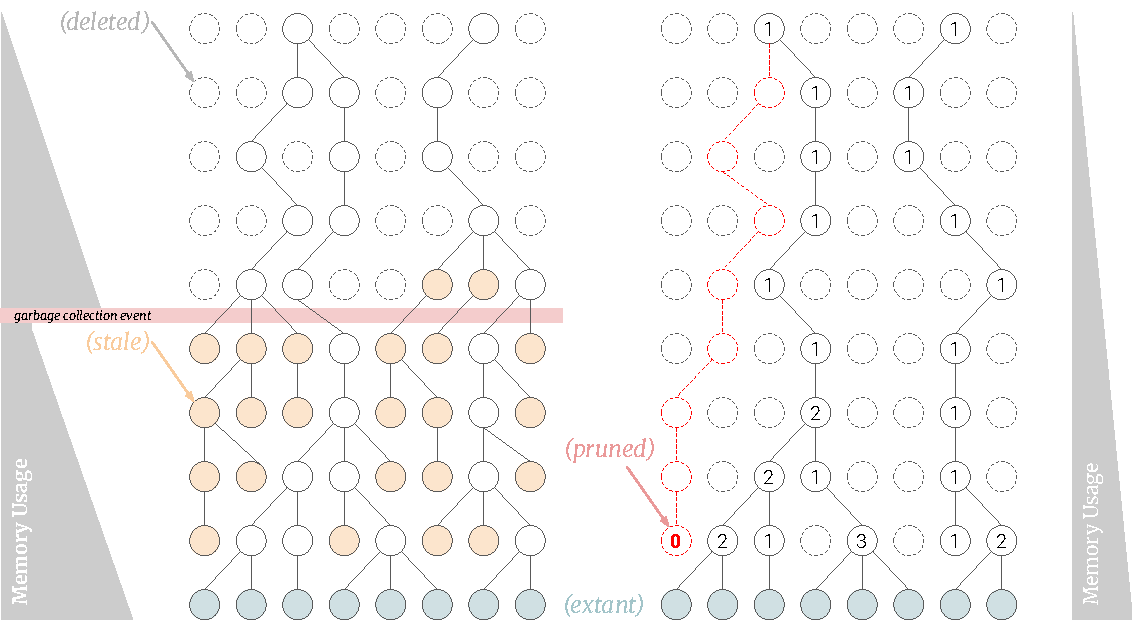
\includegraphics[width=\linewidth]{img/perfect-strategy.pdf}

\begin{minipage}[t]{0.5\linewidth}
  \centering
  \subcaption{garbage collection strategy}
  \label{fig:perfect-strategy:garbage-collection}
\end{minipage}%
\begin{minipage}[t]{0.5\linewidth}
  \centering
  \subcaption{reference counting strategy}
  \label{fig:perfect-strategy:reference-counting}
\end{minipage}
\caption{%
\textbf{TODO.}
TODO.
}
\label{fig:perfect-strategy}
\end{figure}

% TODO

\subsubsection{Time Complexity}

The pruning-enabled algorithm has amortized constant time complexity (see Theorem \ref{thm:perfect-tracking-with-pruning-time}).

\begin{theorem}{Pruning Time Complexity}
\label{thm:perfect-tracking-with-pruning-time}
The time complexity of pruning in perfect phylogenetic tracking is $\mathcal{O}(1)$, amortized. 
\end{theorem}

\begin{proof}
\label{prf:perfect-tracking-with-pruning-time}
The initialization and birth-handling steps of the pruning algorithm are trivially constant-time, as explained in proof \ref{prf:perfect-tracking-time} (technically the pruning algorithm adds two constant-time operations to the birth-handling step, but this fact is inconsequential).

Next, we prove that the removal-handling pruning algorithm runs in amortized constant time.
When an arbitrary taxon $t$ is removed, there are three possibilities: 1) $t$ has living descendants, 2) $t$ has no living descendants, but $t$'s parent is either alive or has other descendants that are alive, or 3) $t$ was the last living descendant of its parent.
In case 1, nothing can be removed from the phylogeny.
Case 1 takes constant time, because it only requires executing a single comparison operation.
In case 2, only $t$ can be removed from the phylogeny.
Case 2 also takes constant time, as it only requires removing a single node from the tree and doing three comparison operations.

In case 3, pruning must be done.
We recurse back up the lineage until we find a taxon, $a$, that is either alive or has living descendants. 
Let the distance between $t$ and the root of the tree be $d_t$ and the distance between $a$ and the root of the tree be $d_a$.
The pruning operation, then, takes $\mathcal{O}(d_t - d_a)$ steps. 
In the worst case, this value will be equal to the number of elapsed generations.

However, for case 3 to occur, all taxa from $t$ to $a$ (including $a$ but not including $t$) must have already been removed.
Consequently, $d_t - d_a$ case 1 removal operations must happen for every case 3 removal operation.
Thus, the amortized time to remove the sequence of taxa from $t$ to $a$ (including both $t$ and $a$) is:

\[
\frac{2(d_t - d_a) + 1}{d_t - d_a + 1}
\]

Since

\[
\lim_{d_t - d_a\to\infty} \frac{2(d_t - d_a) + 1}{d_t - d_a + 1} = 2,
\]

the amortized time complexity of pruning is bounded by a constant, i.e., it is $\mathcal{O}(1)$.


\end{proof}

% TODO: missing proof
% \begin{theorem}{Average Space Complexity of Perfect Tracking with Pruning}
% \label{thm:perfect-tracking-with-pruning-space}
% Average case is best described by the upper-case-lambda coalescent, but math on that is maybe
% less well understood than Kingman coalescent. Kingman coalescent makes a number of more limiting
% assumptions, but most of them are actually fairly appropriate for most phylogeny tracking situations
% (fixed-size population, wright-fisher model). The biggest problem is that it assumes only bifurcations
% (no multi-furcations). However, a strictly bifurcating tree is the worst case for average space complexity
% (a series of non-bifurcating trees is the absolute worst case, but under random selection it would
% quickly turn into a pretty good (best?) case). So, if we can't do an exact proof based on the upper
% case lambda coalescent, we can still do worst average case proof based on the Kingman coalescent
% Oh wait, maybe bifurcations aren't the worst case? Apparently there is a paradoxical result that shows
% that the Kingman Coalescent decreases fastest???

% Okay, here's the thing - all of these different models behave in ways that populations being tracked
% might behave. The argument to make here is that for a ton of them, the size of the tree (Ln) has been
% shown to be constant, proportional to n, limited by some distribution or asymptote, etc. It may even
% be sufficient to say that they come down from infinity. We end up with a space complexity something like
% O(generations + Ln) which in the worst case could translate to something like O(generations + 2*pop_size^2),
% except I think we can actually prove it's actually something more like O(generations + pop_size + log(pop_size))
% slight risk that pop_size should be multiplied by log(pop_size)

% \end{theorem}

% \begin{proof}
% \label{prf:perfect-tracking-with-pruning-space}

% \end{proof}

\subsubsection{Performance in parallel and distrbuted environments}
\label{sec:perfect-tracking-pruning-distrbuted}

% @MAM interesting thought: you can't prune all unifurcations when taking the second (distributed) approach to pruning-enabled perfect tracking
% @MAM another interesting thought: hstrat annotations can be smaller than UUID labels (128 bits)
% TODO: Matthew, double-check this @MAM this is completely reasonable
Like naive perfect tracking, pruning-enabled perfect tracking can proceed via either a fully-centralized database or through localized record-keeping.

Centralized pruning-enabled perfect tracking has all the same issues in parallel and distributed environments that naive perfect tracking has.
It also adds an additional cost: parallel processes must be synced up before a pruning operation can be performed.
Otherwise, the algorithm risks incorrectly pruning a lineage that it will later learn produced a new artifact.
This requirement would translate to a substantial speed cost in practice.

In a localized model, when the last remnant of an immigrant lineage is eliminated an extinction notification would need to be propagated back to the processing element that lineage immigrated from.
Records for lineages that extinct locally but had generated emigres to other processing elements would need to be retained until extinction notifications for all emigres are confirmed.
Even for lineages that span few processing elements, repeat migrations between a single pair of processors could wind up long breadcrumb trails that necessitate extensive cleanup operations.

\subsubsection{Space complexity}
\label{sec:perfect-tracking-pruning-space}

As with naive (i.e., unpruned) perfect tracking, the primary memory cost of pruned perfect tracking comes from maintaining the tree of records, $T$.
Thus, our analysis in this section will focus on the size of $T$.
Technically, the worst-case size order of growth of perfect tracking with pruning is the same as for naive perfect tracking (see Theorem \ref{thm:perfect-tracking-space}).
However, whereas that order of growth is also the best case for naive perfect tracking, it is a somewhat pathological case under pruning.
When using pruning, such a case would only occur when every object is copied before being removed (i.e., no lineages go extinct).
There are some legitimate reasons these cases might occur, but most of them are fairly esoteric (see Section \ref{sec:perfect-tracking-space-supp}).

% These scenarios might legitimately occur if objects are never removed or the number of objects is allowed to continuously grow, but in these cases $N$ would also be growing continuously.
% They could potentially also happen when tracking digital objects that are copied with very small amounts of stochasticity.

With pruning, the asymptotic behavior of the average case turns out to be substantially better than that of the worst case.
Luckily, in the vast majority of applications, the average case is more practically informative than the asymptotic behavior of the worst case.
Here, we investigate the expected size of $T$ (which we will call $E(|T|)$) in the average case as the population size ($N$) and number of time points ($G$) increase.
Of course, investigating the average case requires making some assumptions about the scenarios where this algorithm may be used.
An expedient assumption to make is that objects to be replicated are selected at random from the population (i.e., drift).
This process is described by a neutral model.
While this assumption is obviously not completely true in most cases, it will turn out that $E(|T|)$ is actually smaller for most realistic cases (e.g. any evolutionary scenario with directional selection).

Conveniently, the asymptotic behavior of $E(|T|)$ as $N$ increases has been studied extensively by evolutionary biologists under a variety of random selection models \citep{berestyckiRecentProgressCoalescent2009, tellierCoalescenceMultipleBranching2014, nordborgCoalescentTheory2019}.
The relevant branch of mathematics is coalescence theory, which describes the way particles governed by random processes agglomerate over time.
There are a variety of models of random selection, all of which yield different behavior.

Neutral models that could plausibly describe a process of replicating digital artifacts experience ``coalescence'' events.
In these events, the population establishes a new, more-recent common ancestor as a result of old lineages dying out.
This observation implies that when we run our perfect tracking with pruning algorithm for sufficiently long periods of time, on average we should expect our tree $T$ to have a long unifurcating ``stem.''
The most recent node in this chain will be the most recent common ancestor (MRCA) of the whole extant population.
The descendants of the MRCA will form a sub-tree, which we will call $T_c$.

The expected size of $T_c$ (denoted $E(|T_c|)$ here), then, will be the dominant factor affecting $E(|T|)$.
$E(|T_c|)$ is closely related to a value commonly studied in coalescence theory literature called the expected total branch length (usually denoted $L_n$ or $T_{tot}$; we will refer to it as $L_n$).
$L_n$ assumes that the phylogeny is represented by a tree, $T'$, that contains the leaf nodes, MRCA, and any internal nodes from which multiple lineages diverge (i.e., no unifurcations).
Edges in this tree have weights that represent the amount of time between the origin of the parent and the origin of the child.
$L_n$ is the sum of these weights.
Although the asymptotic behavior of $L_n$ depends on specifics of the evolutionary process, it scales sub-linearly with respect to population size for all realistic models that have been investigated in the literature to our knowledge \citep{gnedinLcoalescentsSurvey2014}.%
\footnote{A possible exception is spatial models, which have received less formal analysis but are known to exhibit slower coalescence \citep{berestyckiRecentProgressCoalescent2009}}
How is this possible?
Under realistic neutral models, various subsets of the population will coalesce to common ancestors much faster than the whole population does \citep{nordborgCoalescentTheory2019}.
Consequently, there are many shallow branches.
The farther back in $T_c$ you go, the fewer branches there are.
As a result, the marginal impact of increasing $N$ diminishes as $N$ increases.

What do these observations tell us about $E(|T_c|)$?
% @ELD Figure here would deifnitely be a good idea
Because $T_c$ contains unifurcations, each edge in $T'$ corresponds to a chain of unifurcating nodes in $T_c$.
The length of this chain in $T_c$ will, on average, be proportional to the weight of the corresponding edge in $T'$.
Thus, the expected value of $L_n$ is almost identical to $E(|T_c|)$.
However, there is one important difference.
The reason $T'$ is able to scale sub-linearly with $N$ is that as $N$ goes to infinity the lengths of the branches to the leaf nodes (i.e., the extant population) approach zero \citep{nordborgCoalescentTheory2019, delmasAsymptoticResultsLength2008, drmotaAsymptoticResultsConcerning2007}.
In contrast, the space taken up by each of the $N$ leaf nodes in $T_c$ is a fixed constant and cannot drop to zero.
Thus, $E(|T_c|)$ is $\mathcal{O}(L_n + N)$.
Note that the time to coalescence depends entirely on the population size ($N$); the total number of generations elasped since the start of the process ($G$) does not affect the asymptotic growth rate of $E(|T_c|)$.

The precise asymptotic scaling of $L_n$ with respect to population size $N$ depends on the exact model of random replication used \citep{tellierCoalescenceMultipleBranching2014}.
Under the best-studied model, Kingman's Coalescent, it is $\mathcal{O}(log(N))$ \citep{kingmanCoalescent1982, delmasAsymptoticResultsLength2008}.
Under another reasonable model, the Bolthausen-Sznitman coalescent, it is $\mathcal{O}(\frac{N}{log(N)})$ \citep{drmotaAsymptoticResultsConcerning2007}.
% Some exotic models could also produce the star-shaped coalescent, in which all $N$ offspring descend directly from the most recent common ancestor.
% While this scenario actually takes less memory in total, its asymptotic growth is $\mathcal{O}(N)$.
Because these growth rates are all less than $N$, $E(|T_c|)$ ends up being dominated by $N$ term.
Thus the overall memory usage of pruning-enable perfect tracking is $\mathcal{O}(N + G)$.
Trivially, the ``stem'' part of $T$ can be pruned off when coalescence occurs, producing a bound of $\mathcal{O}(N)$.

%TODO: This could move to supplement if we need space
While $L_n$ is not the primary factor determining the memory use of this algorithm, it still has a substantial practical impact on resource usage.
Thus, it is worth briefly exploring our practical expectations of its size.
Earlier, we mentioned that in practice $T$ will usually be smaller than predicted by neutral models.
These models represent a scenario called ``neutral drift'' in evolutionary theory.
Under drift, coalescence can be slow because it needs to happen entirely by chance.
When some members of the population are more likely to be selected than others and that selective advantage is heritable (assuming population size $N$ is stable), we expect to see ``selective sweeps'' in which those members of the population outcompete others.
A selective sweep will usually speed up coalescence (unless it is competing with a different simultaneous selective sweep) \citep{neherGeneticDraftSelective2013}.
Thus, in general, in the presence of non-random selection, we expect $T_c$ to be much smaller than we would expect under drift.
Note, however, that the Bolthausen-Sznitman coalescent mentioned above does model scenarios with selection.

Would we ever expect $T_c$ to be larger than under drift?
Only if lineages coexist for longer than we would expect by chance.
Such a regime can theoretically occur when there is selection for stable coexistence or diversity maintenance.
However, such a regime also involves introducing non-random (balancing/stabilizing) selection.
Thus, in practice, while these regimes maintain multiple deep branches, there is often frequent coalescence within those branches.
Theoretically, though, extreme pressure for diversity could cause $E(|T|)$ to scale faster than $\mathcal{O}(N)$.
Such scenarios could potentially be created via ecological interactions.  % TODO cite selection schemes as ecologies?

One factor that we have glossed over in this analysis is the possibility for $N$ to change over time.
For reasons that are explored further in Section \ref{sec:perfect-tracking-space-supp}, allowing population size $N$ to fluctuate complicates mathematical analysis but does not substantially alter our conclusions.


% \section{Main Results} \label{sec:results}

\section{Discussion} \label{sec:discussion}

In choosing between perfect tracking and hereditary stratigraphy, there are multiple factors to consider: 1) time complexity in the relevant model of computation, 2) memory use, and 3) amount of information retained.

\subsection{Time complexity}

In a non-distributed, serial computing environment, perfect tracking runs in constant time.
The time complexity of hereditary stratigraphy depends on the retention policy used, but scales at least linearly with annotation size.
So, if annotation size growth is allowed to maintain static reconstruction resolution guarantees in long-running processes, time complexity of perfect tracking will scale preferably to hereditary stratigraphy.
A lower bound on hereditary stratigraphy's time complexity comes from copying of annotation material from parent to child when new artifacts are born.
Consequently, the exact time complexity depends on the curation policy but can scale with number of generations $G$ elapsed, unless a policy with a constant-cap order of growth is used.
Note that hereditary stratigraphy incurs an additional one-time complexity cost due to the fact that its output generally requires post-processing before analysis (i.e., phylogenetic reconstruction).
Assuming comparable generational depth across lineages, reconstruction can be achieved with time complexity linear to annotation size and linear to tree tip count (which can optionally be held below population size through subsampling).

In contrast, in parallel or distributed environments, perfect tracking suffers from the problems discussed in Sections \ref{sec:perfect-tracking-distrbuted} and \ref{sec:perfect-tracking-pruning-distrbuted}.
Thus, hereditary stratigraphy usually runs faster in these environments and is generally the better choice.
Moreover, it is robust to data loss, making it reliable to use in situations where perfect tracking would break.

\subsection{Memory use}

As discussed in Section \ref{sec:perfect-tracking-pruning-space}, pruning-enabled perfect tracking is fairly memory efficient ($\mathcal{O}(N)$, where $N$ is population size) under a wide range of practical circumstances.
However, in practice, its memory use can vary dramatically over time.
This variation is partially due to the fact that the expected distribution of coalescence times is exponential, leading to substantial variation about the mean.
It is also due to the potential for large variation in tree size caused by the ecological and evolutionary dynamics at play in a given scenario being tracked.
Anecdotally, the memory cost of perfect tracking often poses a real-world obstacle to using it at full resolution.

Like perfect tracking, hereditary stratigraphy's memory footprint grows linearly $\mathcal{O}(N)$ with population size.
Under configurations with guarantee static MRCA resolution at arbitrarily generational depth, memory footprint also scales with $G$ --- either $\mathcal{O}(G)$ or $\mathcal{O}(\log G)$ depending on whether guarantees are absolute or recency-proportional \citep{moreno2024algorithms}.
However, hereditary stratigraphy can also be conducted $\mathcal{O}(1)$ constant with respect to $G$.
Unlike pruning-enabled perfect tracking, hereditary stratigraphy's memory usage is a hard guarantee.
Consequently, it can be a good choice in cases where large fluctuations in memory use are not acceptable.
It can also be helpful in circumstances that inhibit coalescence and start pushing perfect tracking towards worst-case performance.

\subsubsection{Case study: memory use in a distributed environment}

% adapted from https://github.com/mmore500/hstrat-synthesis/blob/8d66ae9240e6c7a6ea00ce3756c8cdf404f9ba45/text/body/introduction.tex#L163-L184
To give a concrete sense of these trade-offs in a distributed setting, consider the memory footprint of pruning-enabled perfect tracking on the Cerebras Wafer-Scale Engine (WSE), a hardware accelerator that provisions each of its many processor elements (PEs) a modest 48kB of memory \citep{cerebras2021wafer}.
In the absence of complex point-to-point communication patterns, identifier values must be kept for each extant lineage emigrating from a memory space --- even if no descendants remain extant locally;
this information remains necessary to ensure an intact breadcrumb trail connecting extant tips back to their founding ancestor.
Although each breadcrumb may individually be small in size --- reasonably 64 bits each, including a generational timestamp --- in aggregate they may accumulate substantially.
To illustrate, consider an island-model population distributed over the WSE processor grid, with 512 individuals resident per PE and neighboring PEs exchanging individuals at a 5\% migration rate.
With a backwards-time coalescent simulator such as msprime, we can estimate the distributed memory footprint of an exact tracking approach incorporating pruning \citep{baumdicker2022efficient}.
Such coalescent simulations sample possible spatio-temporal lineage histories for an extant population.
Using a drift model over structured fixed-capacity subpopulations, we can tractably approximate the full WSE processor grid as 900 independent $30 \times 30$ subgrids.
To account for stochastic variability in sampled lineage histories, we consider memory footprints across 10 independent whole-chip replicates.

Figure \ref{fig:msprime-memory-estimate} compares projected memory footprints between perfect tracking with lineage pruning versus hereditary stratigraphy.
With pruning, the upper bound memory use per PE averages 39.6kB across replicates.
If additional coordination was employed to balance memory load for stored tracking data across PEs, use would be 25.3kB per PE.
Another possible optimization would be periodic checkpoint synchronization with host to export accumulated data.
Batching simulation across 100,000 generation windows in this manner would also reduce memory cost per PE to 25.3kB.
If used together, batching and balancing would require 20.9kB per PE.
As expected, distributed memory footprints for perfect tracking are substantially greater than the 12kB required to store timestamped unique identifiers for perfect tracking in a unified memory space.
Recall that the WSE's 48kB per PE must be shared also among other data records, underlying simulation state (e.g., population genomes), and program data.
Note that the above memory use estimates do not account for transient stale lineage data arising from latency in extinction notifications, do not incorporate safety margins for stochastic variability in lineage histories, and assume that no fossil lineages are archived.
Further, memory cost could increase by orders of magnitude in simulations of sexual populations in order to track lineages of multiple independently-assorting genome sites per individual.

% adapted from https://github.com/mmore500/hstrat-synthesis/blob/8d66ae9240e6c7a6ea00ce3756c8cdf404f9ba45/text/body/introduction.tex#L211-L219
Under hereditary stratigraphy, by contrast, genome information encoding lineage history resides in a single fixed-width annotation, bundled alongside a generation counter.
Memory overhead, therefore, is invariant to lineage history, and can be calculated trivially for a given population size.
Reasonably, 32 bits of annotation data could be used for coarse-resolution inference, 64 bits for moderate-resolution inference, or 256 bits for fine-resolution inference.
With 512 individuals per PE and 32-bit generation counters, total cost sums to 4kB for coarse-resolution inference, 6kB for moderate-resolution inference, and 18kB for fine-resolution inference (Figure \ref{fig:msprime-memory-estimate}).
Compared to distributed perfect tracking with pruning, coarse-resolution hereditary stratigraphy represents a five- to almost ten-fold improvement in memory efficiency (depending on balancing/batching procedures).
Notably, also, memory footprints for coarse- and moderate-resolution inference both weigh in below the practical floor of 12kB required for perfect tracking in a global memory space.

% adapted from https://github.com/mmore500/hstrat-synthesis/blob/8d66ae9240e6c7a6ea00ce3756c8cdf404f9ba45/fig/msprime-memory-estimate.tex
% plot generated by https://github.com/mmore500/hstrat-synthesis/blob/5b892c3ebc8d885467af23164c838b3eb5c0f8e0/binder/2025-10-28-trafficsim_msprime.ipynb
\begin{figure}[h]
\centering
\begin{minipage}{0.62\linewidth}
    \centering
\includegraphics[width=0.95\linewidth]{binder/binder-2025-10-28-trafficsim_msprime.ipynb/binder/teeplots/2025-10-28-trafficsim_msprime/hue=flavor+viz=barplot+x=strategy+y=memory-use-kb+ext=.pdf}
\end{minipage}%
\begin{minipage}{0.38\linewidth}
\caption{%
\textbf{Per-node memory use for phylogeny tracking techniques.}
\footnotesize
Memory estimates for tracking approaches are estimated according to coalescent trees sampled using msprime \citep{baumdicker2022efficient}, to simulate phylogeny migration dynamics across a processor grid.
We assume extinct lineages to be removed from memory through extinction tracking --- meaning that exact records need only be stored for extant lineages (pruning).
We assume unifurcations within the scope of a single PE are collapsed.
For batching optimization, it is assumed that the simulation is halted every 100,000 generations for a clean-up phase where data is offloaded off the chip to free on-chip memory from elapsed history.
For balancing optimization, it is assumed that memory load is shared evenly across the chip so that data capacity is necessary just on behalf of average behavior, not necessarily the most extreme cases requiring a buffer leeway.
Serial direct tracking represents a lower bound on memory usage for a bifurcating phylogeny, which scales as $2N$ for population size $N$.
A population size of 512 agents per node is assumed, with demes arranged in a 2D grid and agents migrating between neighboring demes at a rate of 5\%.
Reconstruction-based estimates assume a hereditary stratigraphy annotation of the indicated size, bundled with a 32-bit generation counter.
}
\label{fig:msprime-memory-estimate}
\end{minipage}
\end{figure}


\subsection{Accuracy}

% TODO unifurcations?
As its name implies, perfect tracking returns completely accurate phylogenetic data.
Nevertheless, memory use can be tuned by increasing the granularity of data being recorded (i.e., make the taxonomic unit represented by each node more abstract).

Hereditary stratigraphy introduces imprecision that can potentially lead to inaccuracy.
At the same time, it introduces tools for precisely controlling the level of inaccuracy and its trade-off with memory and time costs.
As such, it can provide more granular scaleback of phylogenetic resolution than is possible through coarsening of taxonomic units under perfect tracking.
Hereditary stratigraphy is always tracked at the level of the individual (i.e., maximum taxonomic resolution), meaning it can capture phylogenetic events that perfect tracking would have to lump together due to memory constraints.

%TODO: Plug ALife paper if its not already in reconstruction

\subsubsection{Overall take-away}

Perfect tracking and hereditary stratigraphy are complimentary techniques that occupy different methodological niches.
In many simple cases, perfect tracking requires fewer resources and provides more accurate data.
However, hereditary stratigraphy can operate in computational environments that perfect tracking cannot.
It also enables new trade-offs to be made between data resolution, memory use, and data accuracy.
Lastly, while perfect tracking is often more memory efficient, hereditary stratigraphy can be configured to provide strong $\mathcal{O}(1)$ guarantees about memory use.

% Considerations:
% - Distributed vs. not
%     - data loss
%     - have to eventually collect data into a centralized representation?
%     - have to propagate extinction notifications during experiment (unlike phylogeny collation which could hypothetically occur after the fact)
% - Accuracy
% - Memory fluctuations


% \section{Experimental Evaluation} \label{sec:experimental-evaluation}

TODO: add content from alife paper here


\section{Conclusion} \label{sec:conclusion}

% Phylogenetic analysis of digital evolution systems provides a cinch application for ancestry trees estimated via hereditary stratigraphy, but other possibilities include tracking message propagation in distributed systems or content propagation in distributed social networks.
% To this end, we report a trie-based algorithm to enable ancestry tree reconstructions comprising large numbers of artifacts.

% ELD: TODO: I think this should maybe go in the conclusion?
% Although envisioned first-and-foremost as application-oriented tool for experiment instrumentation, this line of thinking also presents something of an intriguing curiosity.
% Typically, phylogeneticists tailor algorithms to the demands of available data, not the other way around.
% This notion invites deeper consideration of phylogenetic information encoding within genomes.
% For example, it would be interesting to explore upper bounds on phylogenetic reconstruction accuracy given genome length for different generational depths and population sizes.

We have documented the algorithmic backing of both direct phylogenetic tracking and the emerging ``hereditary stratigraphy'' methodology for distributed lineage tracking of replicating digital artifacts.
% This method works by annotating replicating entities with a heritable annotation, and then comparing end-state annotations after the fact to estimate their phylogenetic relationships --- akin to how biologists infer phylogenetic relationships from biological sequences.
% We have shown the underlying mechanism of hereditary stratigraphy to be an instance of a more general ``streaming curation'' problem.
% This problem requires online subsampling of a rolling observation stream to balance requirements to maintain information over stream history and to limit the number of retained observations.
% In addition to hereditary stratigraphy, the streaming curation problem is faced in use cases involving memory-constrainged data logger or wiresless sensor network devices.
% We identify five policy algorithms that provide different size/coverage trade-offs for the streaming curation problem, and provide procedures to enact them efficiently.

With respect to hereditary stratigraphy, we have here focused on the postprocessing algorithms used to compare and interpret hereditary stratigraphic annotations.
In particular, we present a trie-based tree reconstruction algorithm that proceeds from the underlying structure of the hereditary stratigraphic annotation.
As a point of comparison, we provide an algorithmic formalization of the established perfect-tracking algorithms currently standard in agent-based evolutionary modeling.
We find that both perfect tracking and hereditary stratigraphy have circumstances in which they excel.
%Hereditary stratigraphy enables tracking in noisy, parallel, and distributed environments where perfect tracking would be impractical.
%It also makes stoner guarantees about memory use (although on average perfect tracking uses less memory than most hereditary stratigraphy policies).
%Lastly, it allows different tradeoffs between data resolution, accuracy, and memory use.
%TODO talk about the take away of comparing the two
% ELD: Took a stab at it

% Much future work remains.
% We are particularly interested in adapting hereditary stratigraphy to even more effectively make use of space in fixed-capacity contexts and minimize rearrangement of strata in the underlying annotation data structure (e.g., array of strata) during the update process.
% One promising direction involves adapting retention policies to directly specify the index positions to replace rather than the deposit times of strata to prune.
% Additionally, more general applications of the streaming curation problem would be worth exploring more directly.
% There is also more theoretical analysis to be done.
% Most notably, through the lens of information theory it would be possible to conduct a more formal analysis of the information-retention trade-offs among different policy algorithms.
% This work would also open the door to a more precise analysis of the relationship between pairwise relatedness estimation accuracy and overall tree reconstruction quality.
% Finally, it would be worth assessing the extent to which curation policy algorithms minimize the number of records necessary to achieve their guarantees.

Ultimately, our interest in extraction of phylogenetic history is application-driven.
To these ends, reference implementations of most algorithms described are provided in the public-facing \texttt{hstrat} and \texttt{phylotrackpy} Python libraries \citep{moreno2022hstrat, dolson2023phylotrackpy}.
These libraries enable application of perfect phylogenetic tracking and hereditary stratigraphy techniques in a few lines of code.



% \section*{Acknowledgment}

This research was supported in part by NSF grants DEB-1655715 and DBI-0939454 as well as by Michigan State University through the computational resources provided by the Institute for Cyber-Enabled Research.
This material is based upon work supported by the Eric and Wendy Schmidt AI in Science Postdoctoral Fellowship, a Schmidt Futures program.


\putbib


\end{bibunit}

\clearpage
\newpage

\setcounter{section}{0}
\makeatletter
\renewcommand \thesection{S\@arabic\c@section}
\renewcommand\thetable{S\@arabic\c@table}
\renewcommand \thefigure{S\@arabic\c@figure}
\makeatother

\begin{bibunit}

\section{Appendix}

\printunsrtglossary[numberedsection=autolabel]

\subsection{Additional notes on the memory requirements of perfect tracking} \label{sec:perfect-tracking-space-supp}
% TODO: section name that isn't monstorously long

Note that perfect phylogeny tracking algorithms are designed to plug into a larger computational process.
For phylogeny tracking to be relevant, this computational process must have a collection of $N$ objects that are currently eligible to be copied (in evolutionary terms, the population).
Therefore, the space complexity of this process must be at least $\mathcal{O}(N)$.
As long as the expected size of $T$ scales no faster than $\mathcal{O}(N)$, then, phylogeny tracking will not be the primary factor determining memory usage.
While the memory cost of phylogeny tracking could still be significant in these cases, it is unlikely to be the primary factor determining whether running the program is tractable.

Previously, we noted that cases where perfect tracking with pruning achieves its worst-case size order of growth are esoteric.
There are two ways that these situations can occur:

\begin{enumerate}
\item $N$ is continuously increasing.
\item There is effectively no coalescence.
\end{enumerate}

In case 1, the space complexity of the external computational process will also be growing at least as fast as $\mathcal{O}(N)$.
Because $N$ itself is growing, this behavior should overwhelm the size of the history in $T$ in most cases.
Even in the (completely unrealistic) case where $N$ is allowed to reach infinity, there is an argument to be made that the internal nodes of $T$ would not be substantially contributing to memory complexity.
While this argument is beyond the scope of this paper, it would center around the fact that most evolutionarily realistic coalescence processes ``come down from infinity'' \citep{berestyckiRecentProgressCoalescent2009}.
% Indeed, unless $N$ starts out infinite, any process observed by phylogenetic tracking must come down from infinity, as they 

Case 2 is a legitimate circumstance where worst-case memory complexity could occur. 
It would occur in cases where every member of the population has (approximately) one offspring.
While this level of regularity is unlikely in the context of evolution, it could happen when tracking non-evolutionary digital artifacts.

% \subsection{Extant Record Size Order of Growth of Retention Policy Algorithms} \label{sec:extant_record_oog}
% The concept of `extant record order of growth' is defined to be the upper bound of memory usage of a policy algorithm with respect to elapsed generations.
% Since policy algorithms determine the strata retained into the following generation without the use of any additional data structures, the upper bound of their memory usage will be equivalent in order to the number of retained strata.
% In fact, given that no intermediate data structures other than the final output array are used, we can guarantee the lower bound will also be equivalent.

% As such, Extant Record Size Order of Growth proofs will set out to prove that the number of retained strata of each respective retention policy algorithm will grow with an order of $\mathcal{\theta}(f(n, k)),$ where $f$ is unique to each retention policy algorithm, $k$ is a user-defined constant and $n$ is the number of strata in the current generation.





\putbib


\end{bibunit}

\end{document}
